% =====================================================================
%  DSP391m · Group 5 — Exploratory Data Analysis (standalone deck, English)
%  CCNU-style Beamer (matches Task3_Slides_CCNU_EN). Compile with Tectonic.
% =====================================================================
\documentclass[aspectratio=169,10pt]{beamer}

\usetheme{Madrid}
\usecolortheme{beaver}
\setbeamertemplate{navigation symbols}{}
\setbeamertemplate{caption}{\insertcaption}

\usepackage{iftex}
\ifPDFTeX
  \usepackage[T1]{fontenc}\usepackage[utf8]{inputenc}\usepackage{lmodern}
\else
  \usepackage{fontspec}
\fi
\usepackage{booktabs}\usepackage{array}\usepackage{tabularx}\usepackage{colortbl}
\usepackage{graphicx}\graphicspath{{../figures/}{figures/}{./}}
\usepackage{tikz}\usepackage{pgfplots}\pgfplotsset{compat=1.18}
\usetikzlibrary{arrows.meta,positioning}

\definecolor{ccnured}{HTML}{C00000}
\definecolor{ccnudark}{HTML}{7A0E12}
\definecolor{ccnunavy}{HTML}{31318A}
\definecolor{rowtint}{HTML}{F4ECEC}

\setbeamercolor{frametitle}{fg=ccnured,bg=black!6}
\setbeamercolor{title}{fg=ccnured}
\setbeamercolor{structure}{fg=ccnured}
\setbeamercolor{section number projected}{bg=ccnunavy,fg=white}
\setbeamercolor{itemize item}{fg=ccnunavy}
\setbeamercolor{itemize subitem}{fg=ccnured}
\setbeamercolor{block title}{bg=ccnunavy,fg=white}
\setbeamercolor{block body}{bg=ccnunavy!8}
\setbeamerfont{frametitle}{series=\bfseries}
\setbeamertemplate{section in toc}[ball]
\setbeamertemplate{blocks}[rounded][shadow=true]

\newcolumntype{Y}{>{\raggedright\arraybackslash}X}
\newcommand{\hc}[1]{{\bfseries\color{white}#1}}
\newcommand{\tcode}[1]{{\ttfamily #1}}
\newcommand{\takeaway}[1]{\vspace{2pt}\par{\footnotesize\itshape #1}}
\newcommand{\keynum}[1]{\vspace{2pt}\par{\small\textcolor{ccnured}{$\blacktriangleright$ \textbf{Key:}}\ #1}}

\AtBeginSection[]{\begin{frame}{Outline}\tableofcontents[currentsection]\end{frame}}

\title[EDA]{Exploratory Data Analysis (EDA)}
\subtitle{OULAD — Time-Aware Explainable Early At-Risk Prediction · Data Tasks}
\author[Group 5 -- DSP391m]{Group 5 -- DSP391m}
\institute[FPT University]{FPT University}
\date[DSP391m 2026]{Data Science Capstone (DSP391m) \textbullet{} Report 2}

% footer label
\makeatletter
\setbeamertemplate{footline}{%
  \leavevmode\hbox{%
  \begin{beamercolorbox}[wd=.5\paperwidth,ht=2.4ex,dp=1ex,leftskip=.6em]{author in head/foot}%
    \usebeamerfont{author in head/foot}Group 5 -- DSP391m (FPT University)\end{beamercolorbox}%
  \begin{beamercolorbox}[wd=.3\paperwidth,ht=2.4ex,dp=1ex,center]{title in head/foot}%
    \usebeamerfont{title in head/foot}Exploratory Data Analysis\end{beamercolorbox}%
  \begin{beamercolorbox}[wd=.2\paperwidth,ht=2.4ex,dp=1ex,right,rightskip=.6em]{date in head/foot}%
    \usebeamerfont{date in head/foot}\insertframenumber\,/\,\inserttotalframenumber\end{beamercolorbox}}}
\makeatother

\begin{document}

\begin{frame}[plain]\titlepage\end{frame}
\begin{frame}{Table of Contents}\tableofcontents\end{frame}

% =====================================================================
\section{Setup \& Pipeline Context}
% =====================================================================
\begin{frame}{Where EDA Sits in the Pipeline}
  \begin{columns}[T]
    \begin{column}{0.5\textwidth}
      \footnotesize
      \begin{itemize}\setlength\itemsep{0.35em}
        \item EDA runs \textbf{after cleaning}, on the analysis-ready \tcode{master\_raw} (\textbf{32,593 $\times$ 33}).
        \item Inputs: \tcode{master\_raw} (t=100\%) for univariate / bivariate / correlation; the \textbf{6 checkpoint datasets} for the time-aware analysis.
        \item EDA is not decoration — it \textbf{feeds three downstream decisions}:
        \begin{itemize}\setlength\itemsep{0.1em}
          \item feature handling (which to \tcode{log1p} / keep),
          \item the \textbf{leakage check} (no $|r|\geq0.95$),
          \item the \textbf{RQ1 checkpoint schedule} (when the signal is usable).
        \end{itemize}
      \end{itemize}
      \keynum{descriptive $\to$ univariate $\to$ bivariate $\to$ multivariate $\to$ time-aware.}
    \end{column}
    \begin{column}{0.5\textwidth}
      \centering
      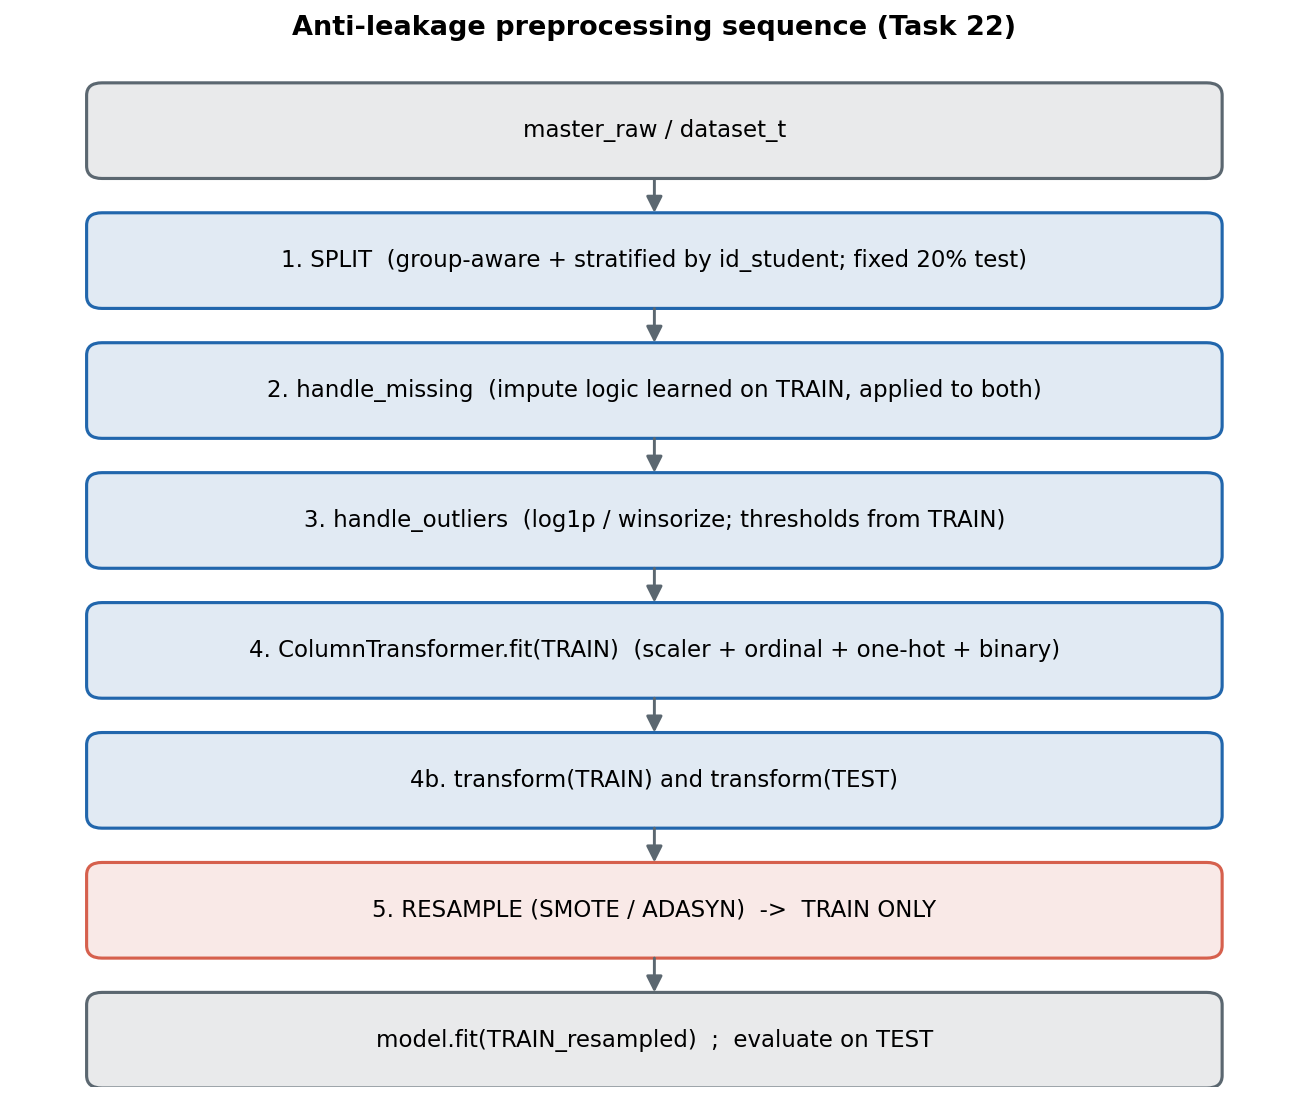
\includegraphics[width=\linewidth,height=0.72\textheight,keepaspectratio]{preprocessing_sequence.png}\\
      {\scriptsize\itshape EDA informs steps 2–5 of the preprocessing sequence.}
    \end{column}
  \end{columns}
\end{frame}

\begin{frame}{EDA Objectives \& Data Profile}
  \footnotesize
  \begin{itemize}\setlength\itemsep{0.3em}
    \item \textbf{Understand} the data: 32,593 students, 33 variables, three groups — Demographic \textbullet{} Engagement \textbullet{} Performance.
    \item \textbf{Check quality}: missing values, variable types, outliers.
    \item \textbf{Find} features that separate at-risk vs not-at-risk students (the core question).
    \item \textbf{Serve two decisions}: feature selection \& leakage control.
  \end{itemize}
  \keynum{32,593 records \textbullet{} 33 columns \textbullet{} 3 feature groups; quality after cleaning: \textbf{0 NaN} in feature columns, 0 duplicate keys.}
\end{frame}

% =====================================================================
\section{Univariate Analysis}
% =====================================================================
\begin{frame}{Numeric Distributions (Histogram + KDE)}
  \begin{columns}[T]
    \begin{column}{0.58\textwidth}\centering
      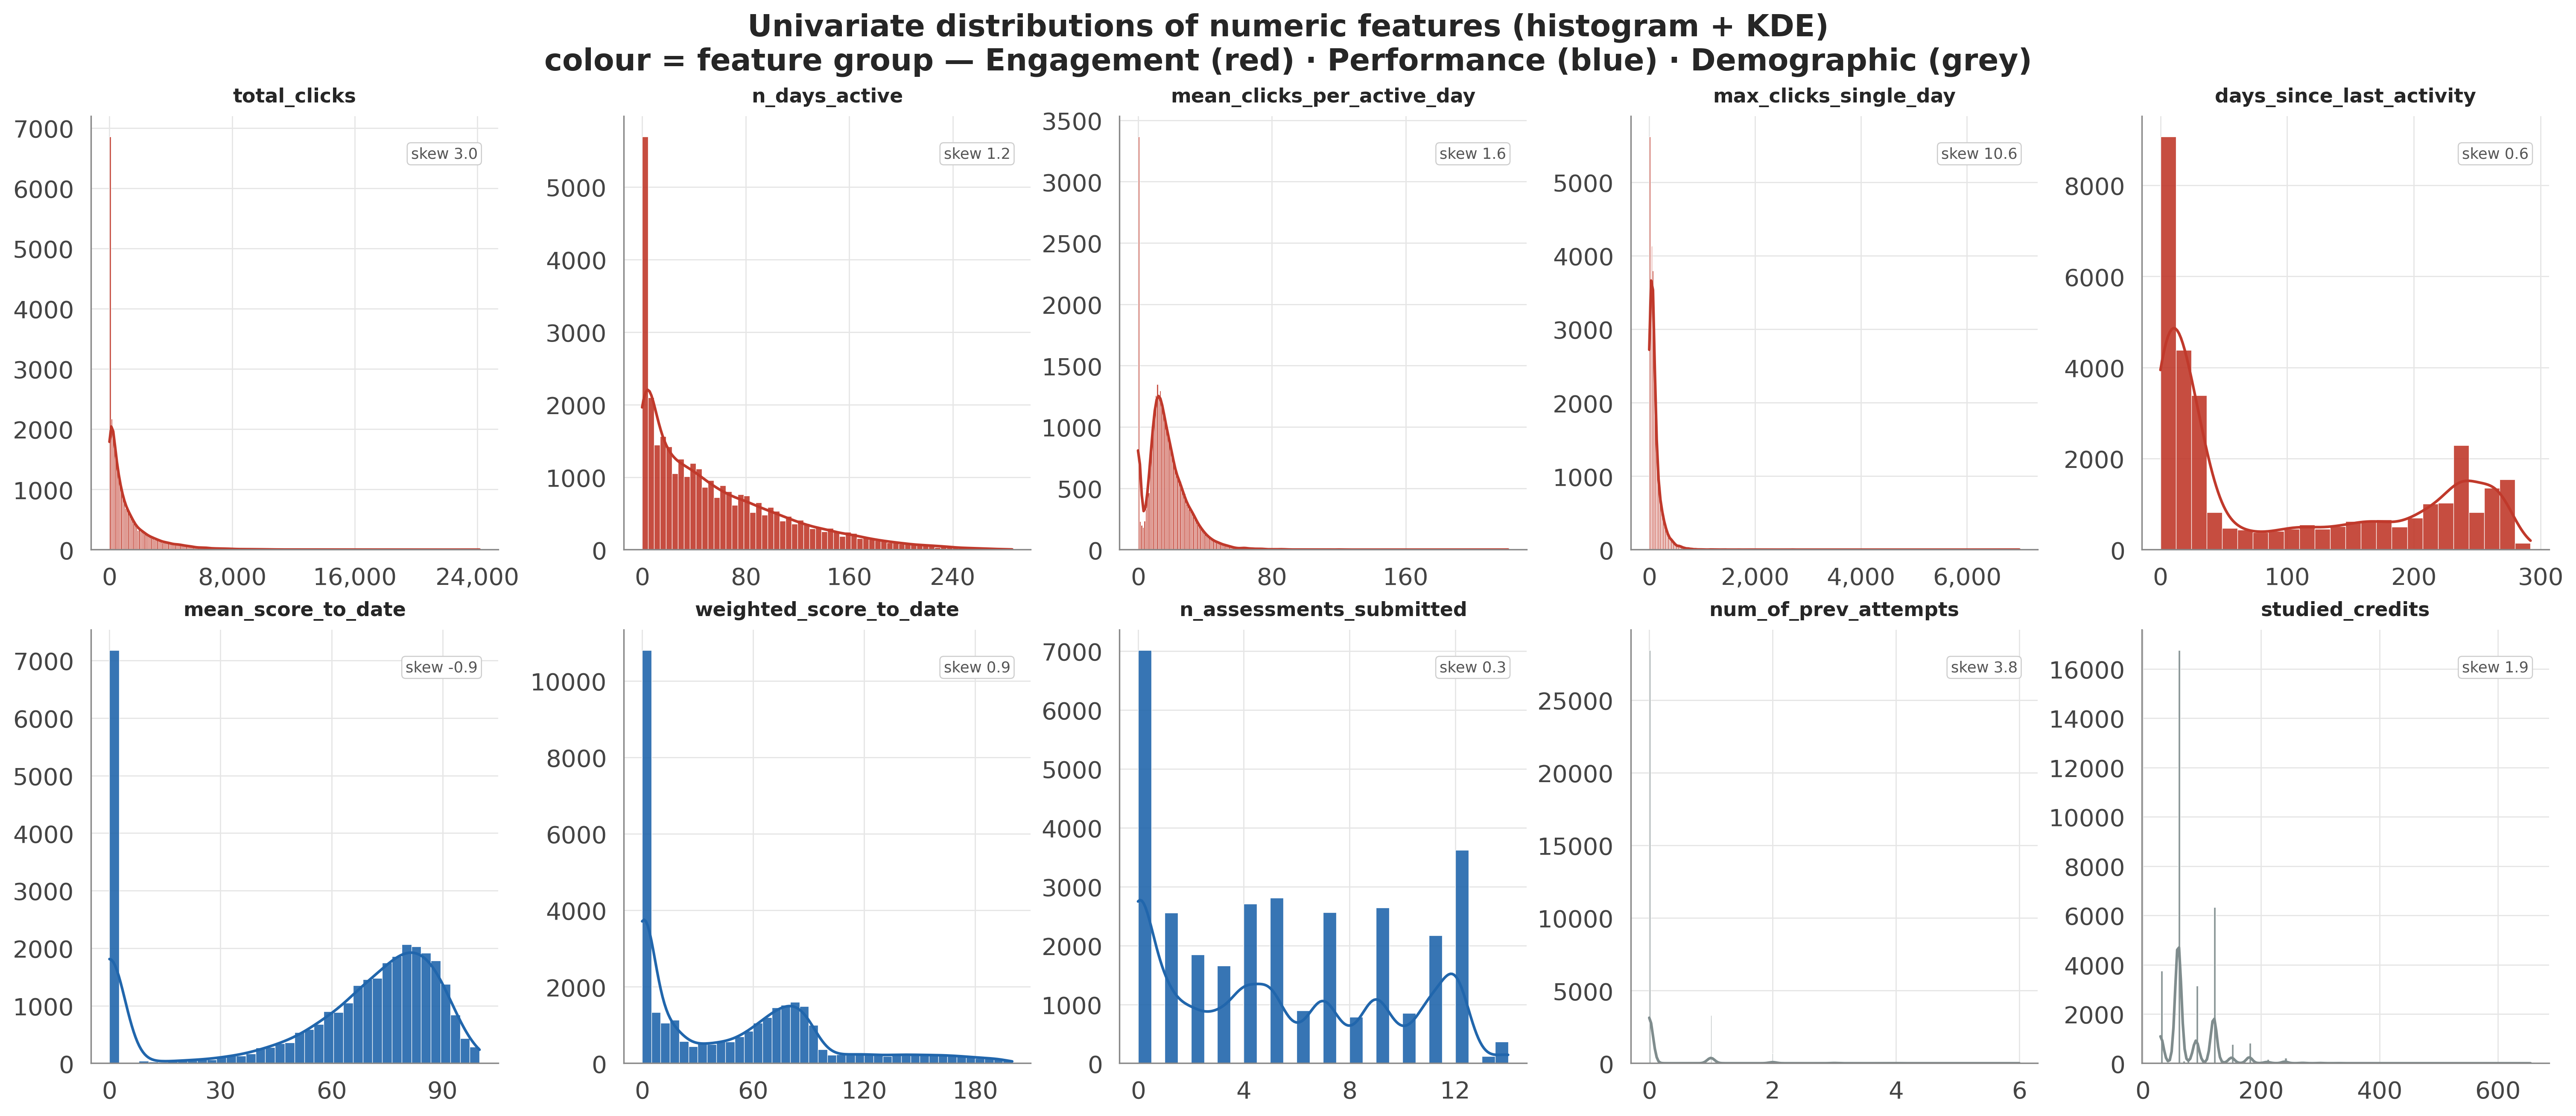
\includegraphics[width=\linewidth,height=0.76\textheight,keepaspectratio]{univariate_hist_kde.png}
    \end{column}
    \begin{column}{0.42\textwidth}\footnotesize
      \begin{itemize}\setlength\itemsep{0.3em}
        \item Most clickstream features are \textbf{strongly right-skewed}: \tcode{clicks\_resource} skew \textcolor{ccnured}{34.7}, kurtosis $\approx$2,125.
        \item Heavy tails are \textbf{real} (super-active students) $\Rightarrow$ \tcode{log1p}, not deletion.
        \item \tcode{days\_since\_last\_activity} is \textbf{bimodal} — the disengagement signature.
        \item Non-normal $\Rightarrow$ non-parametric \textbf{Mann–Whitney} downstream.
      \end{itemize}
    \end{column}
  \end{columns}
\end{frame}

\begin{frame}{Boxplots — Spread \& Skew}
  \begin{columns}[T]
    \begin{column}{0.62\textwidth}\centering
      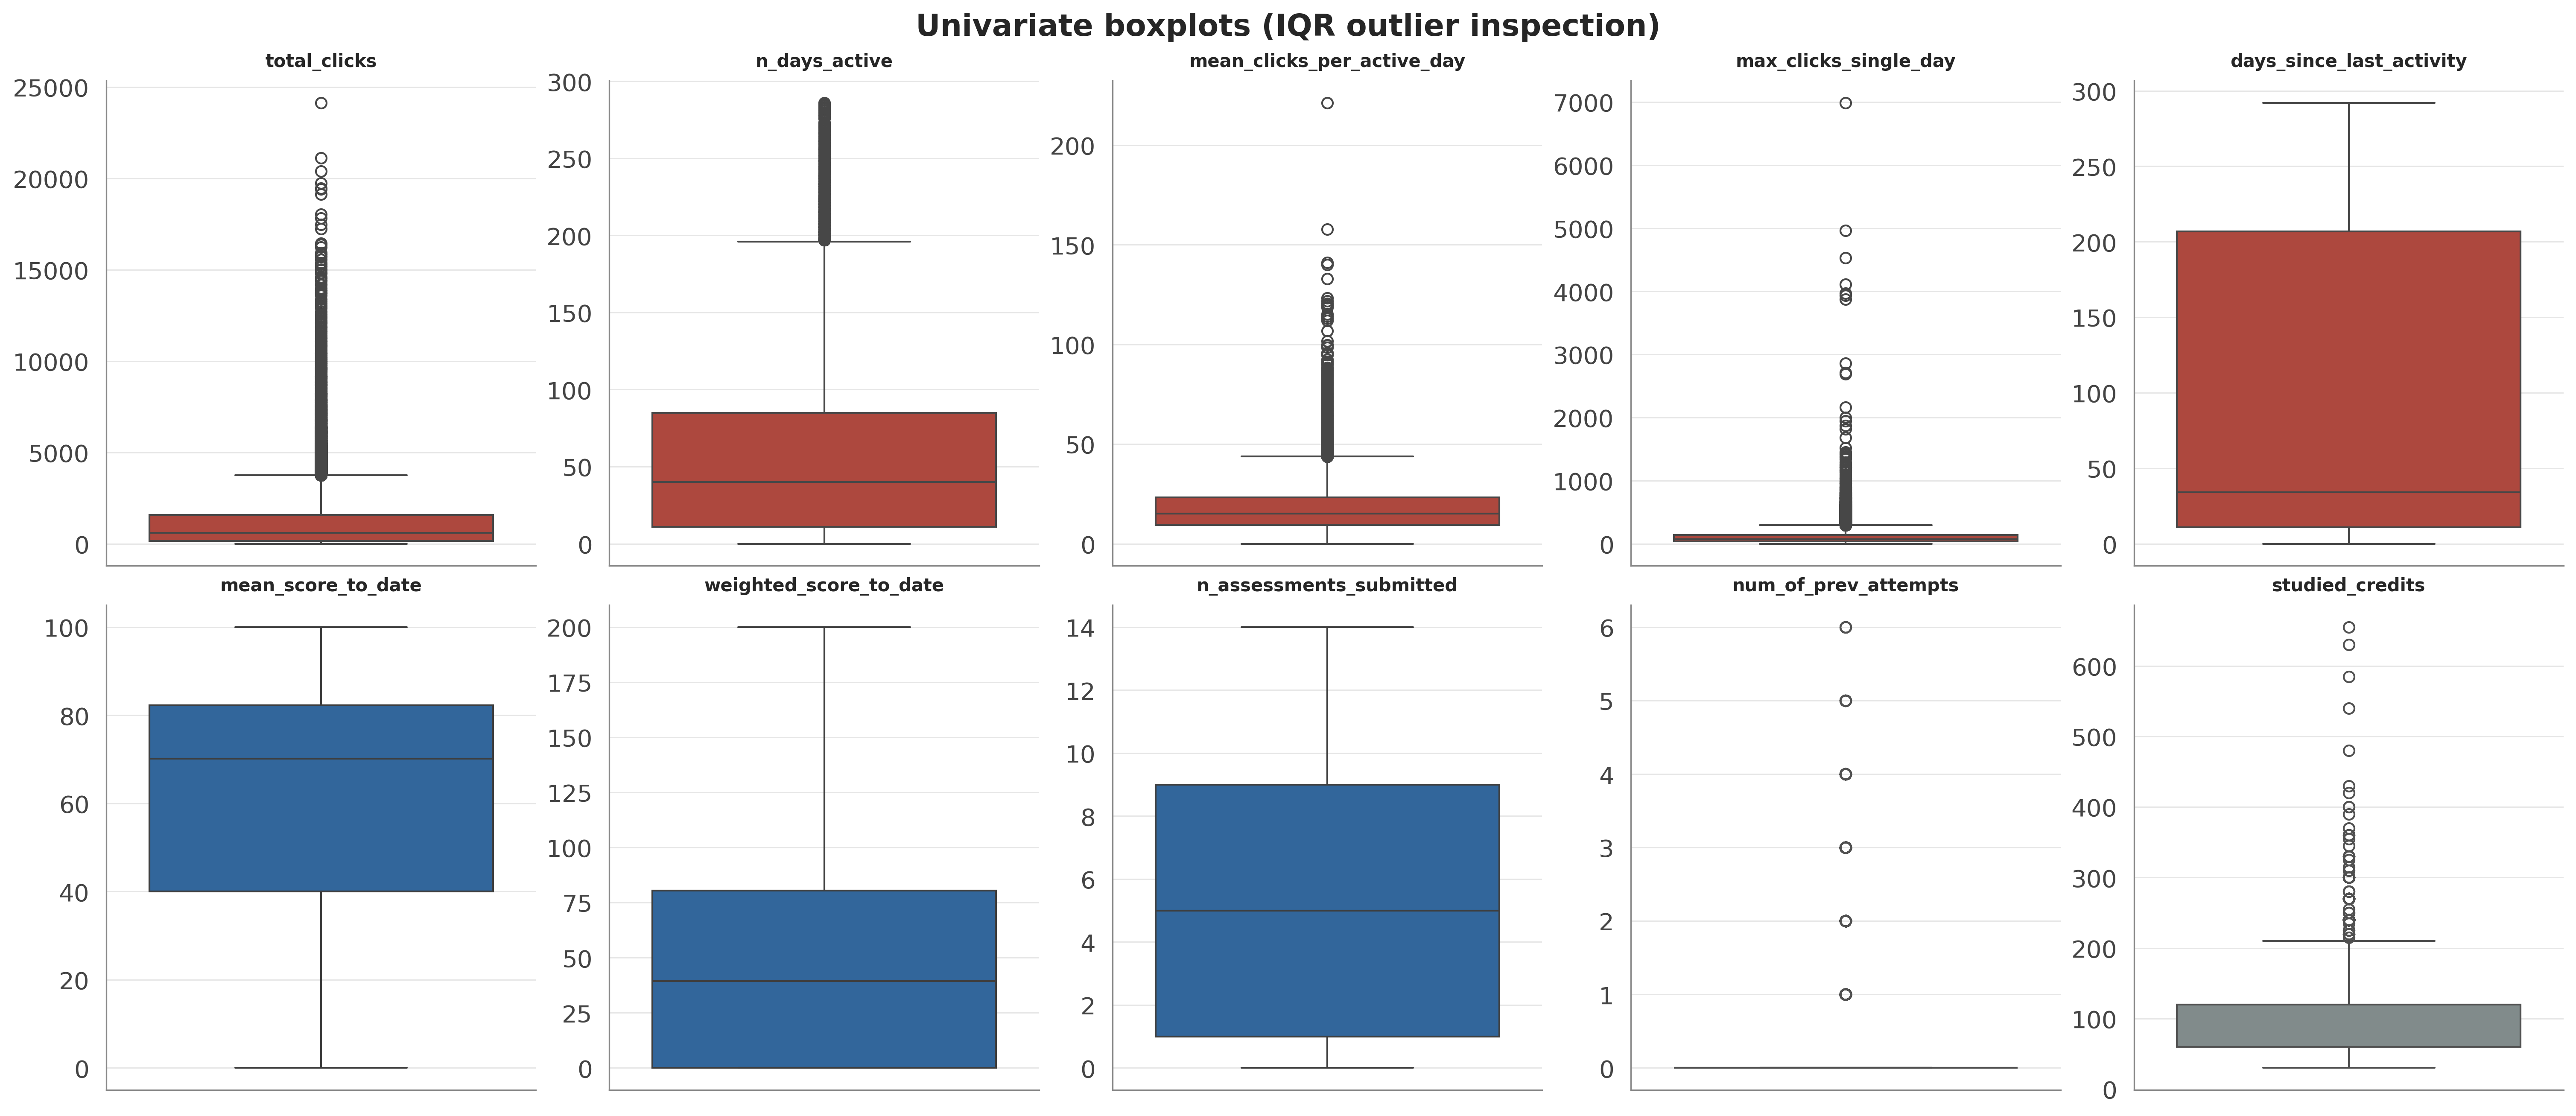
\includegraphics[width=\linewidth,height=0.76\textheight,keepaspectratio]{univariate_boxplots.png}
    \end{column}
    \begin{column}{0.38\textwidth}\footnotesize
      \begin{itemize}\setlength\itemsep{0.3em}
        \item IQR rule confirms long right tails on every click feature.
        \item \tcode{max\_clicks\_single\_day} reaches \textcolor{ccnured}{6,988} vs a small median.
        \item Treatment: \tcode{log1p} (clicks) \textbullet{} winsorise 1\% (bounded) \textbullet{} none (already bounded) — \textbf{no row deleted}.
      \end{itemize}
    \end{column}
  \end{columns}
\end{frame}

\begin{frame}{Categorical Frequency}
  \begin{columns}[T]
    \begin{column}{0.62\textwidth}\centering
      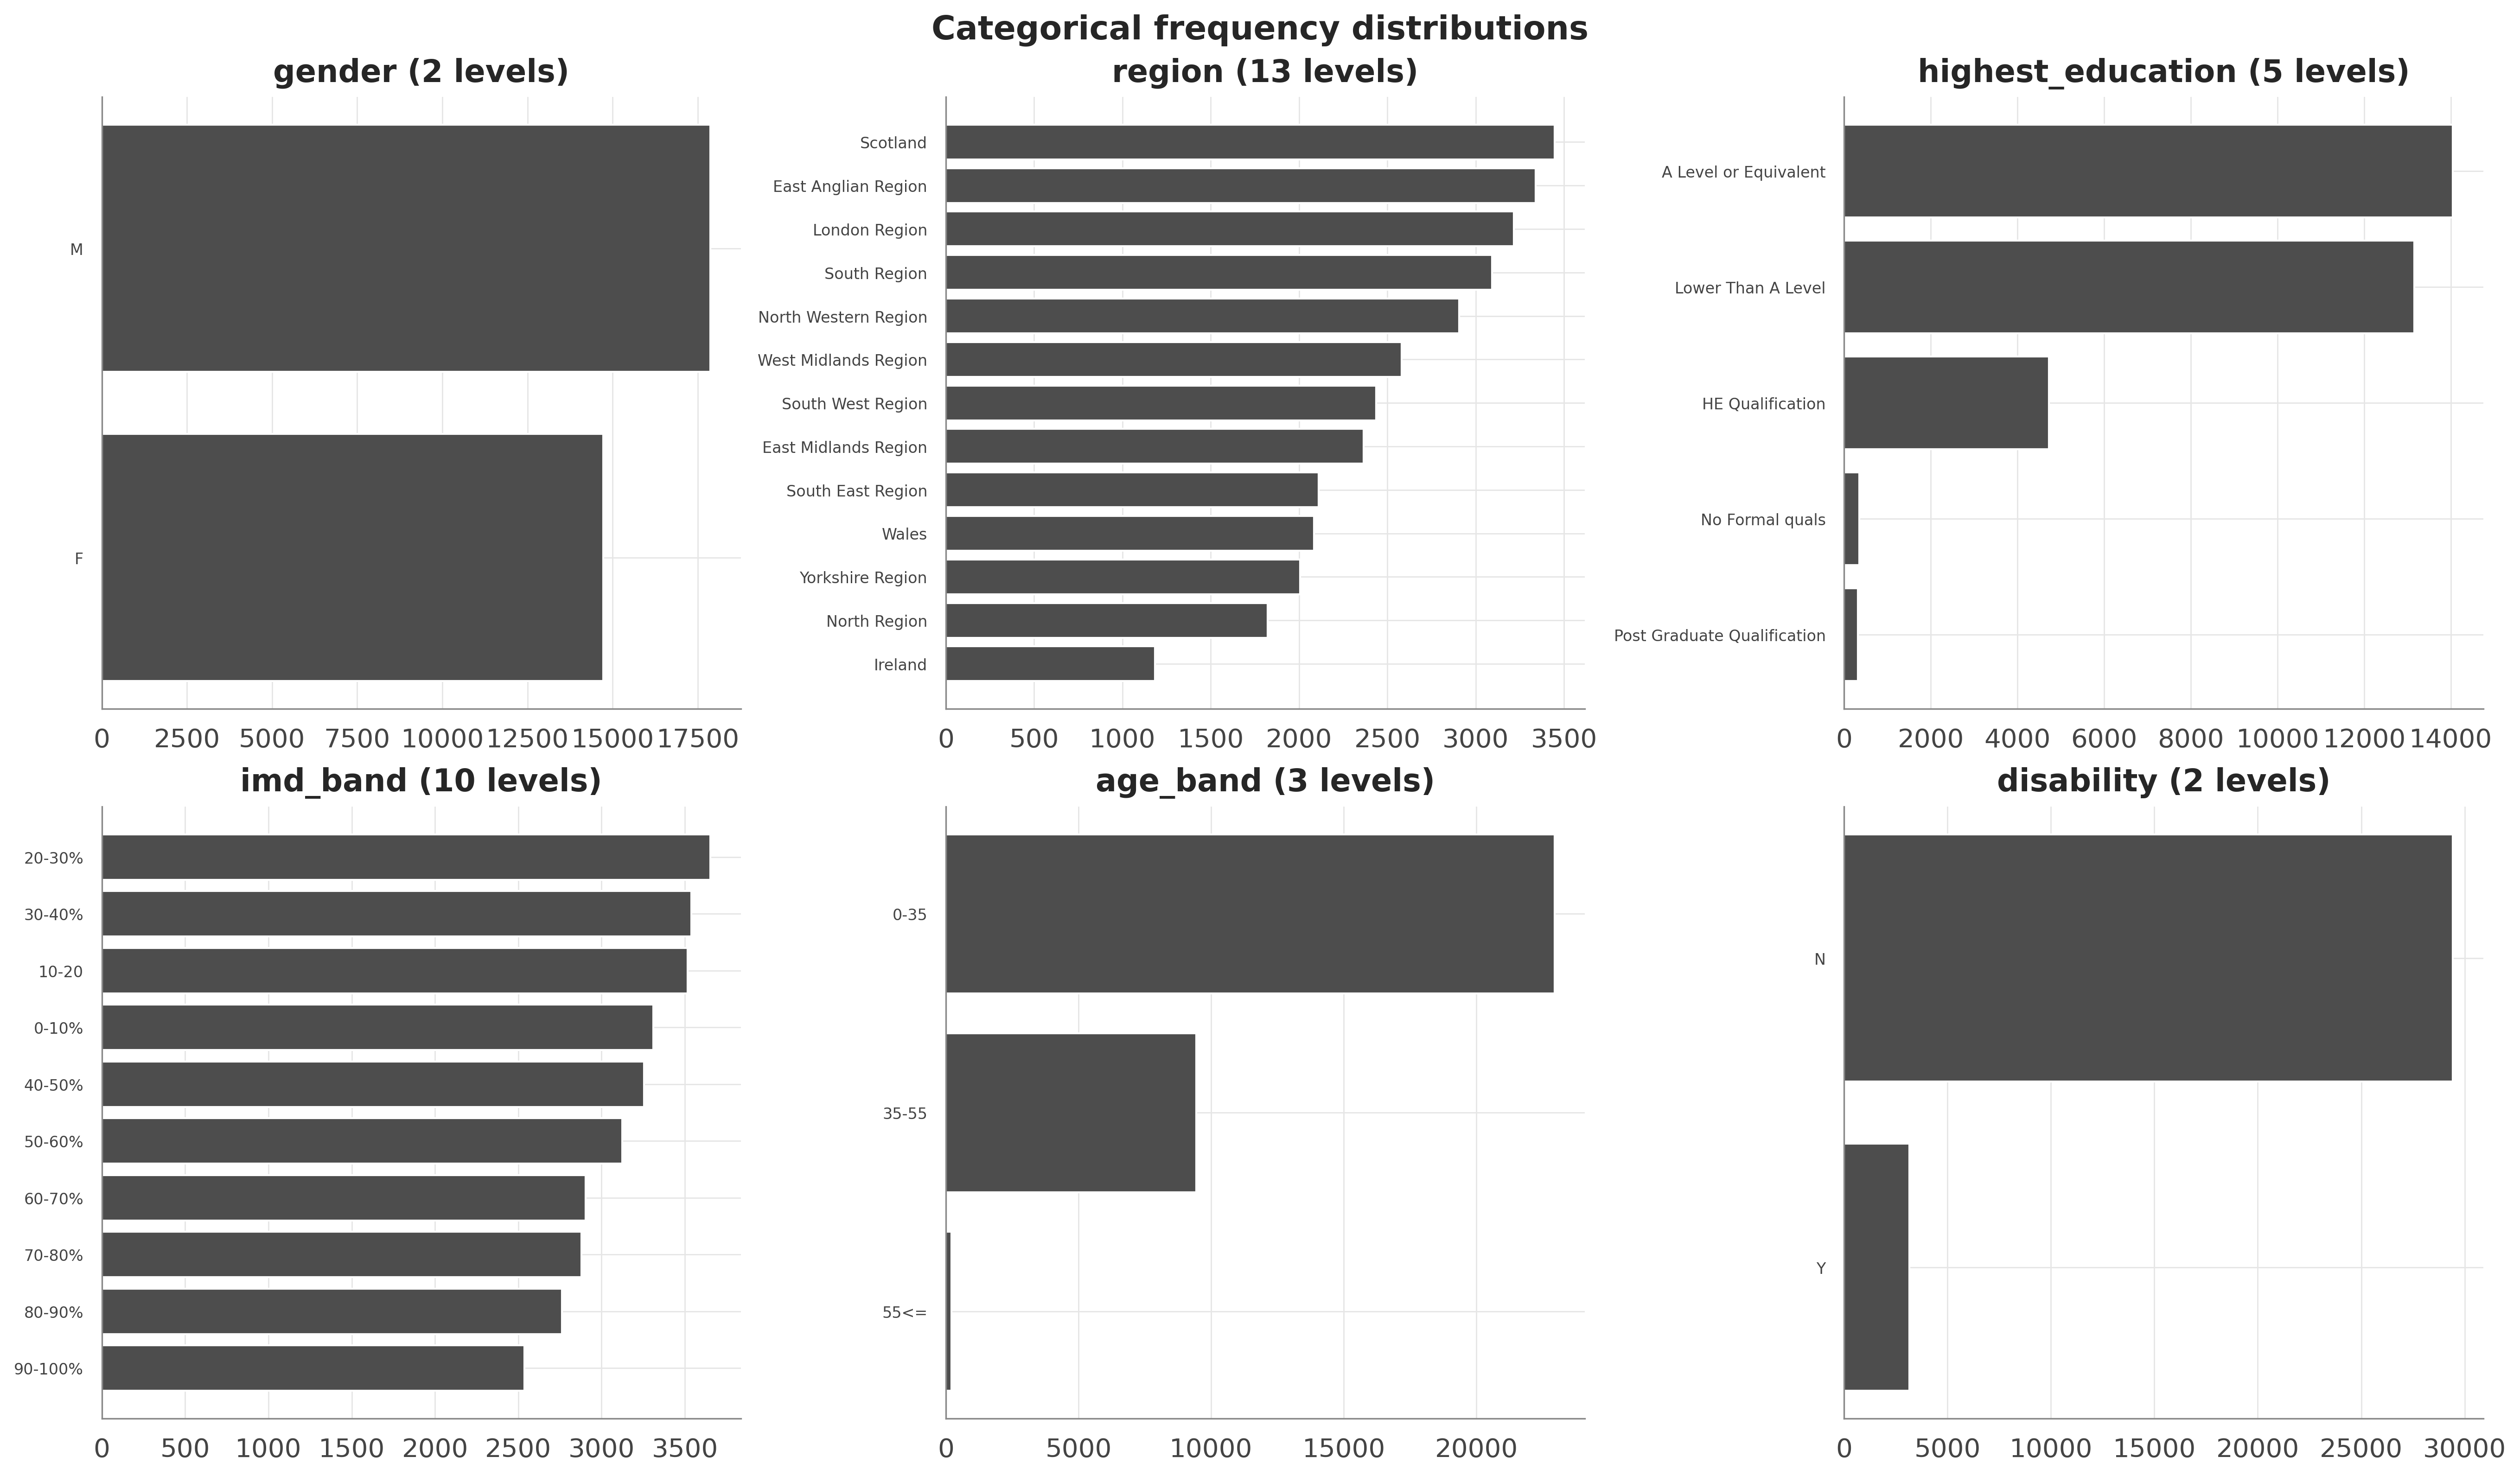
\includegraphics[width=\linewidth,height=0.76\textheight,keepaspectratio]{univariate_categorical_freq.png}
    \end{column}
    \begin{column}{0.38\textwidth}\footnotesize
      \begin{itemize}\setlength\itemsep{0.3em}
        \item \textbf{83\%} of students hold A-Level or below.
        \item Post-Graduate \& No-Formal are \textbf{rare} ($<$1.1\% each).
        \item Rare levels $\Rightarrow$ one-hot with \tcode{handle\_unknown=ignore}, not dropping.
      \end{itemize}
      \takeaway{Imbalanced categoricals shape the encoding choice (Part 4).}
    \end{column}
  \end{columns}
\end{frame}

\begin{frame}{Target Distribution \& Class Balance}
  \begin{columns}[T]
    \begin{column}{0.58\textwidth}\centering
      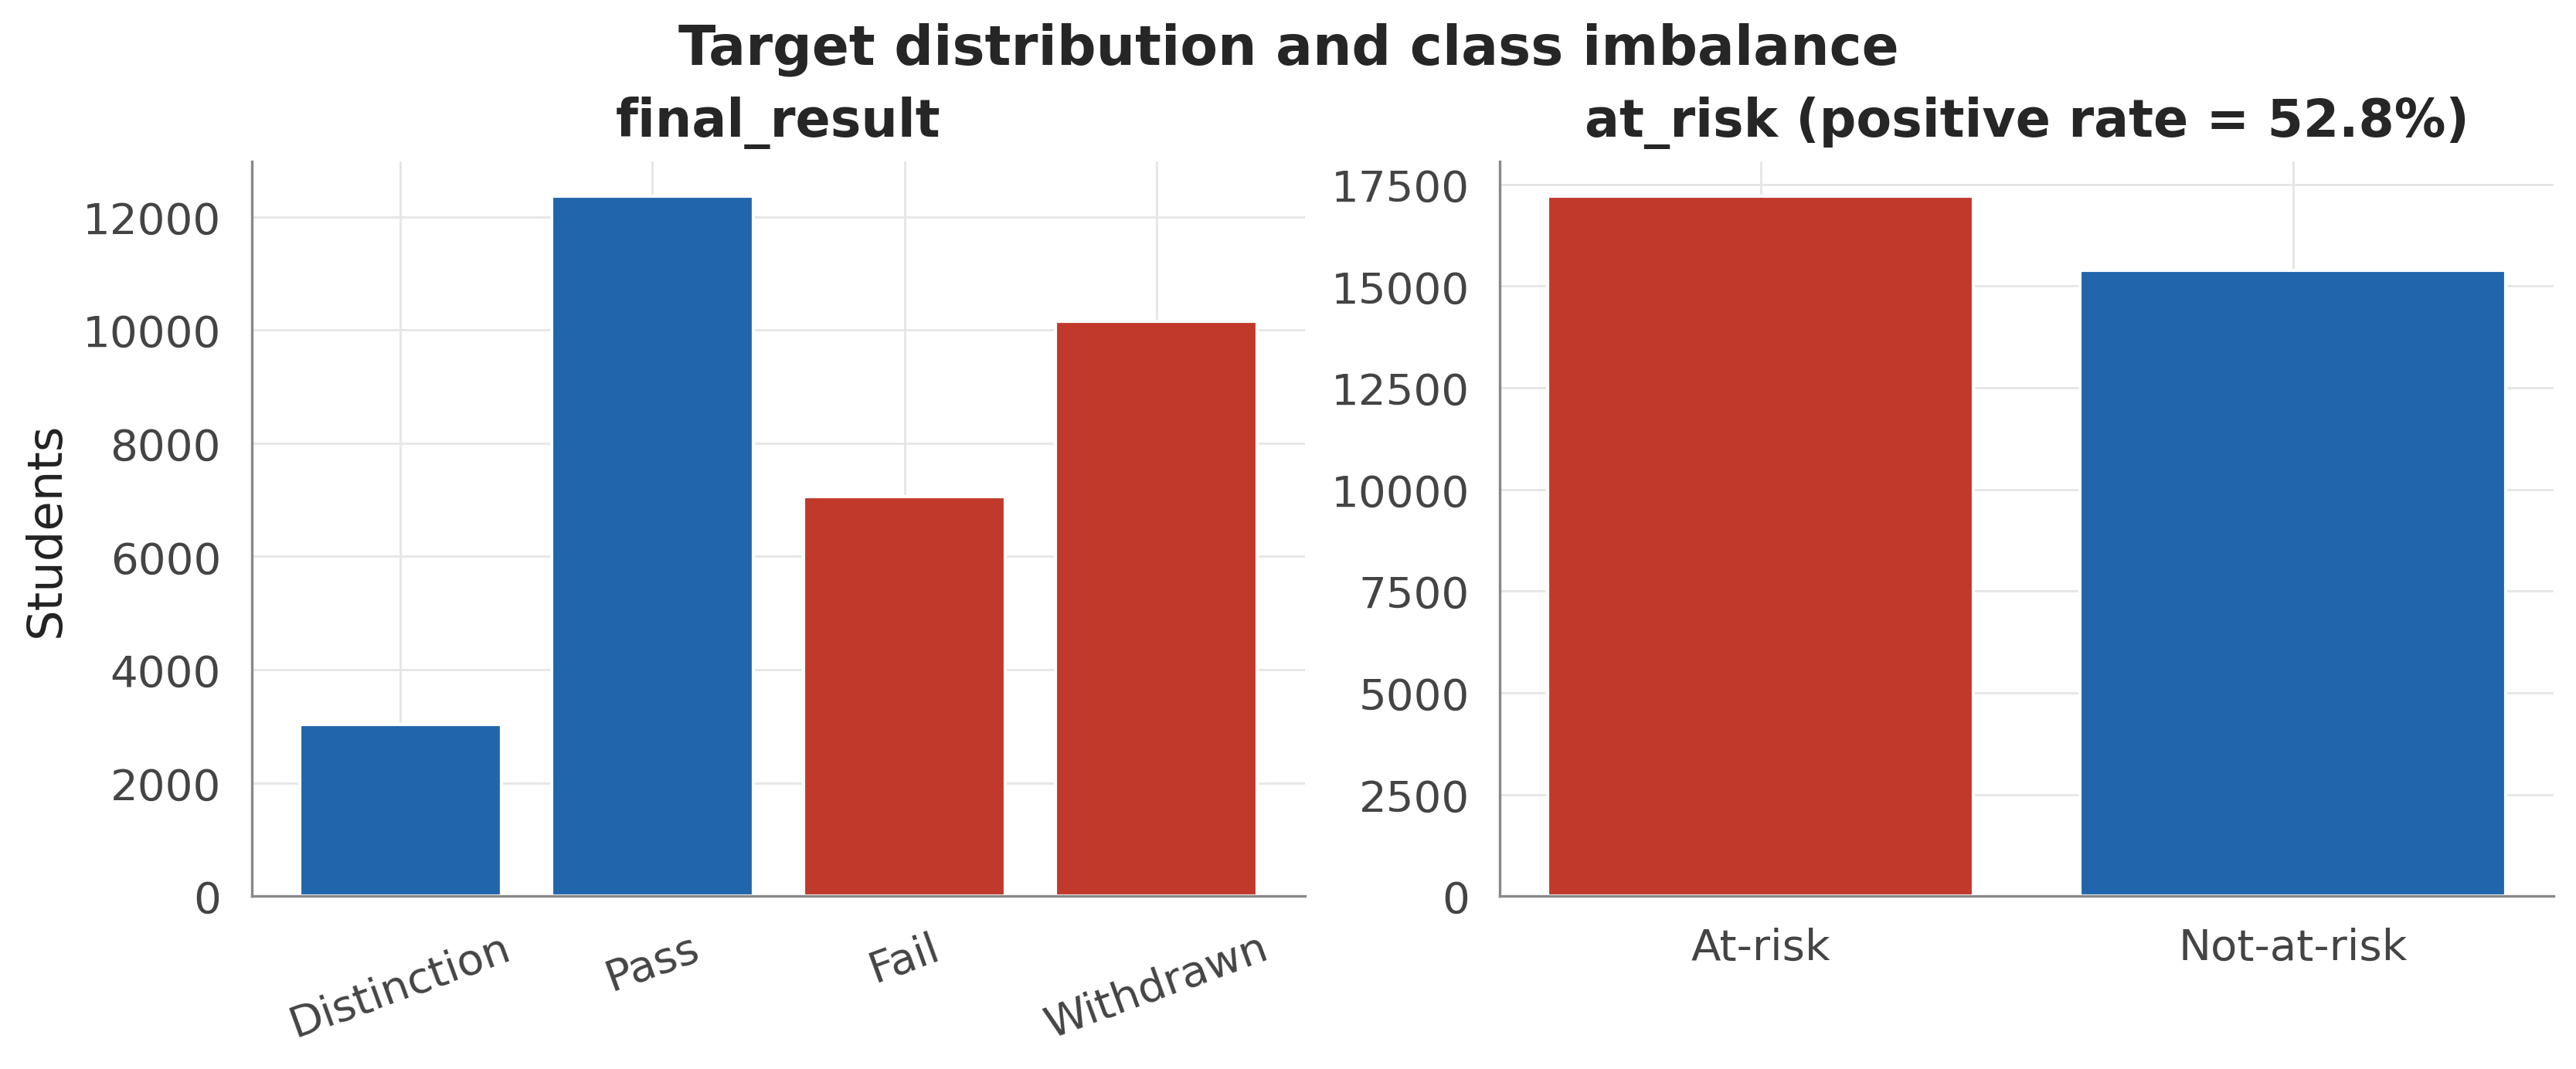
\includegraphics[width=\linewidth,height=0.74\textheight,keepaspectratio]{target_distribution.png}
    \end{column}
    \begin{column}{0.42\textwidth}\footnotesize
      \tcode{at\_risk = final\_result $\in$ \{Fail, Withdrawn\}}
      \begin{itemize}\setlength\itemsep{0.3em}
        \item At-risk \textbf{52.8\%} (17,208) vs not-at-risk 47.2\% (15,385) — \textbf{mild} imbalance (ratio 1.12).
        \item \textbf{Withdrawn} is the largest single class.
        \item Metrics: \textbf{PR-AUC} + \textbf{recall} on the at-risk class.
      \end{itemize}
    \end{column}
  \end{columns}
\end{frame}

% =====================================================================
\section{Bivariate Analysis (vs at-risk)}
% =====================================================================
\begin{frame}{Numeric Features vs At-Risk (Cohen's $d$)}
  \begin{columns}[T]
    \begin{column}{0.54\textwidth}\centering
      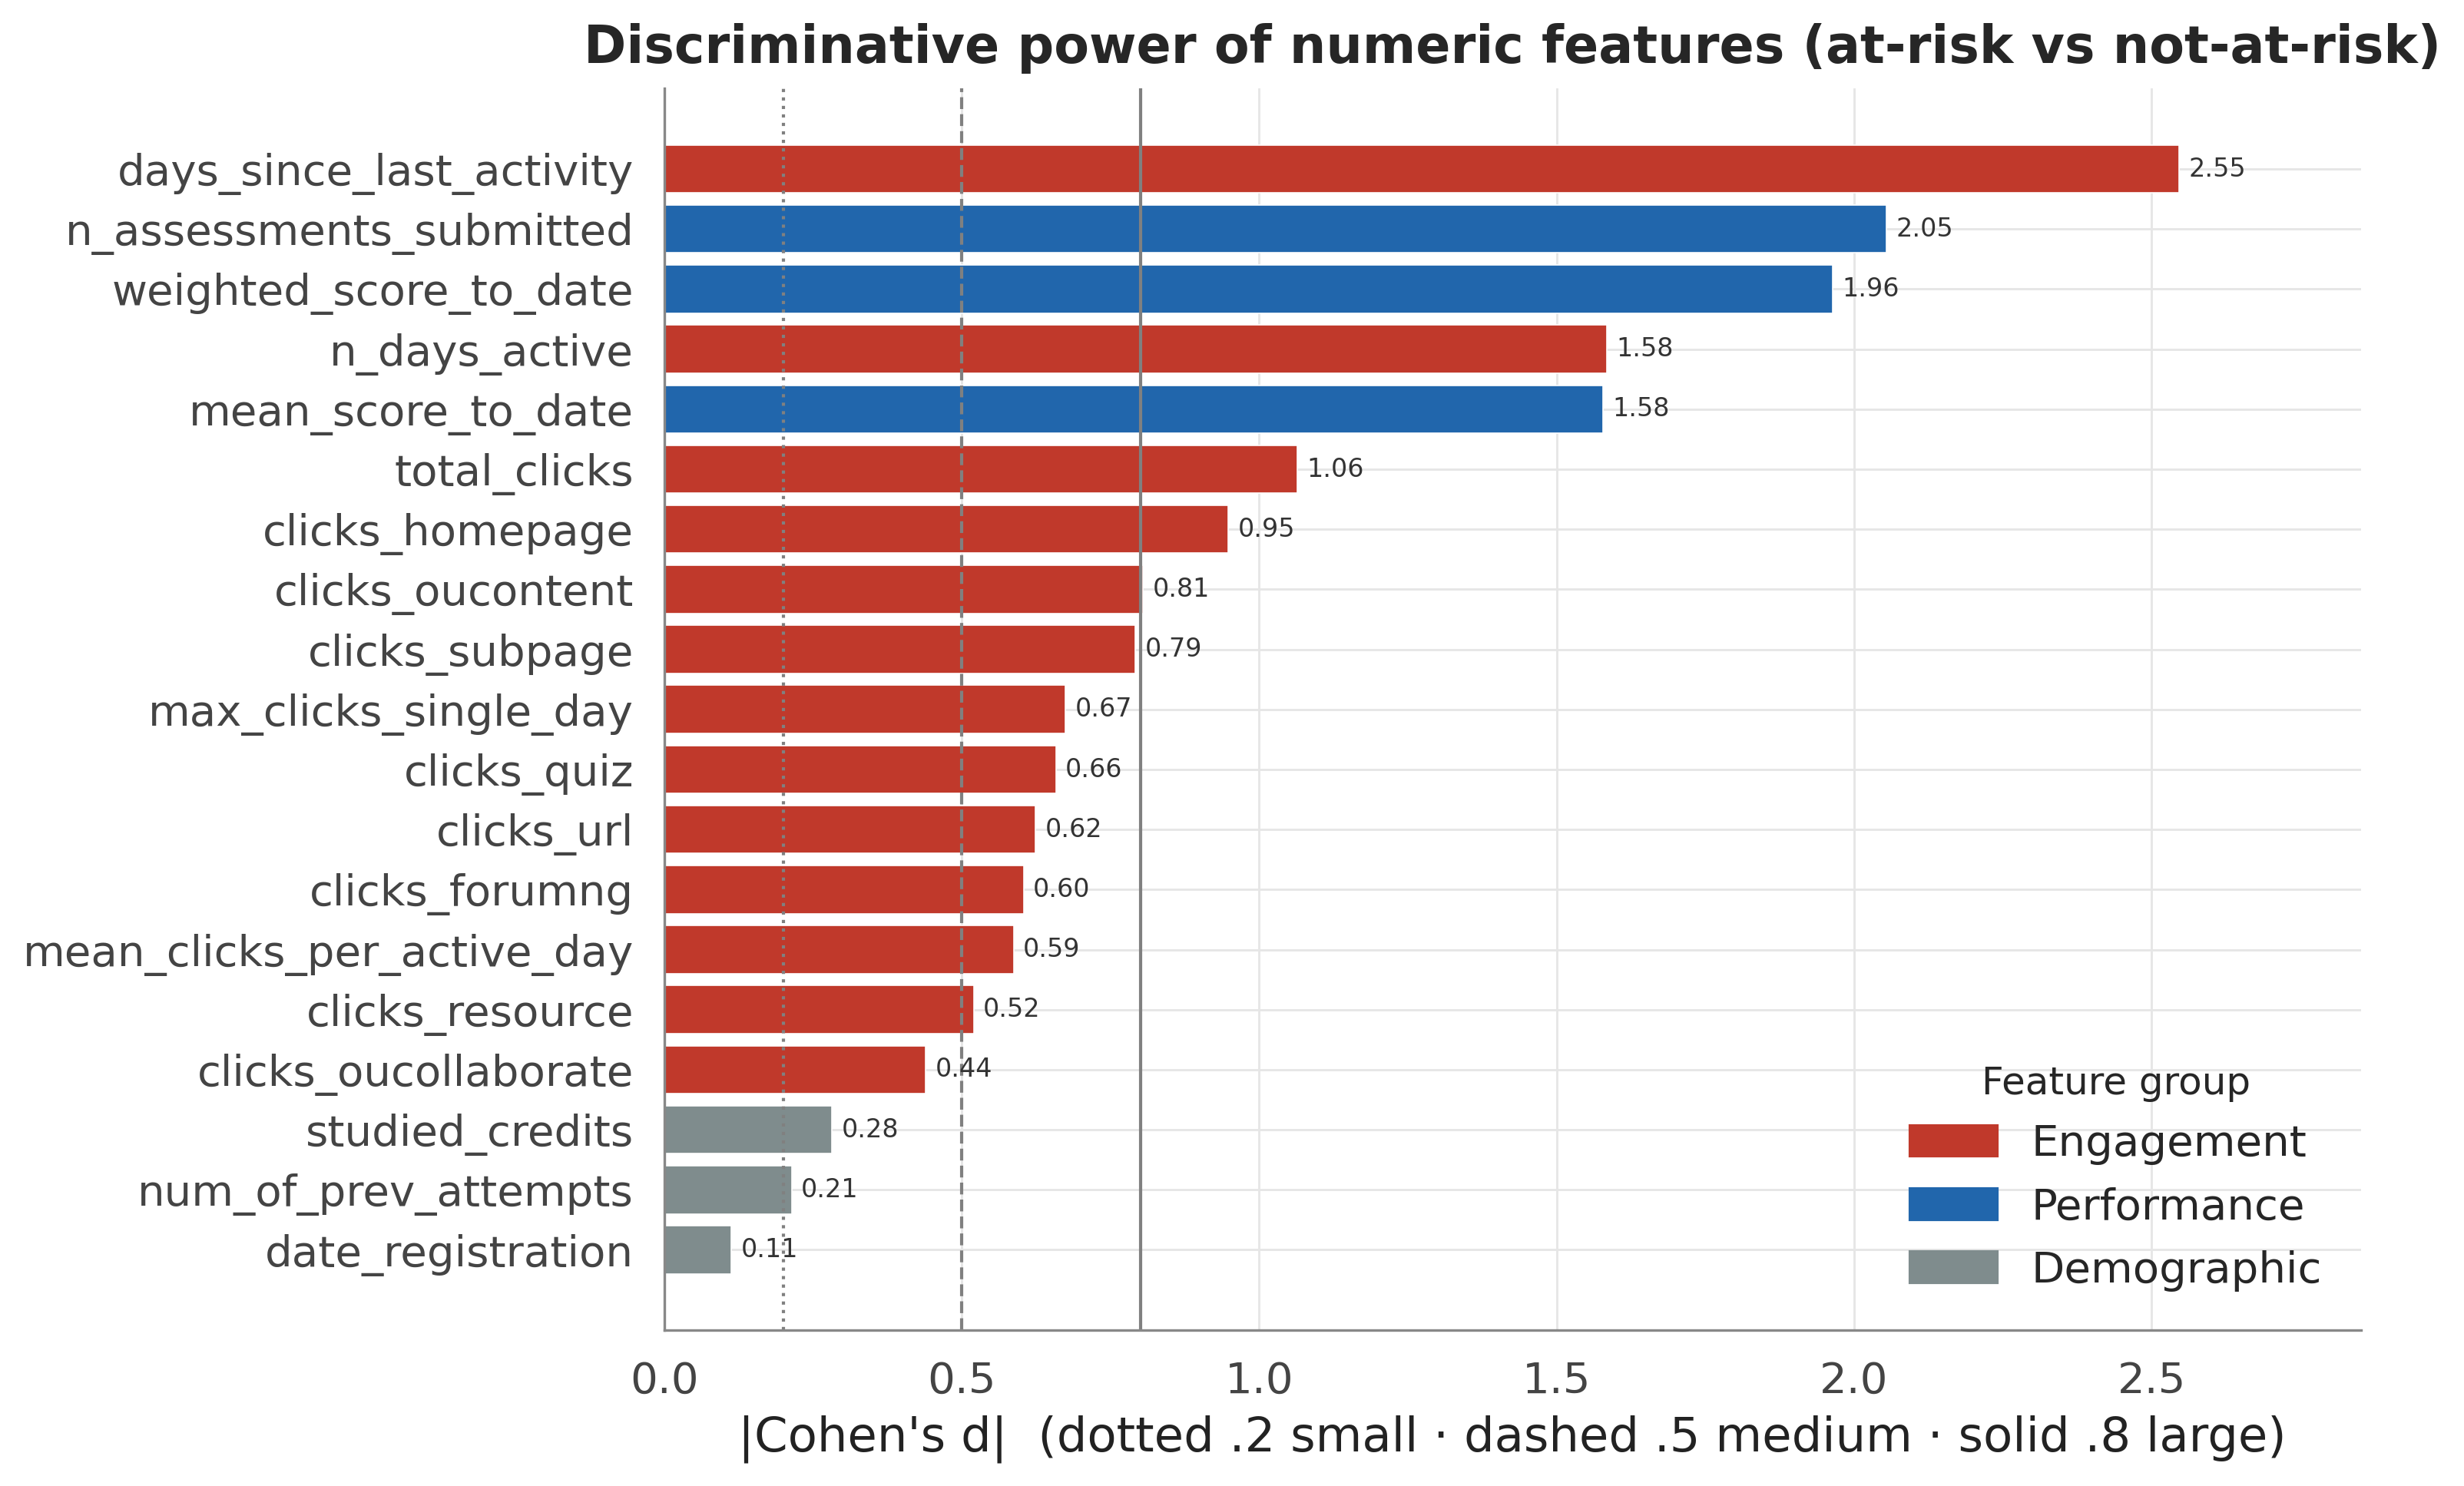
\includegraphics[width=\linewidth,height=0.78\textheight,keepaspectratio]{bivariate_effect_sizes.png}
    \end{column}
    \begin{column}{0.46\textwidth}\footnotesize
      \begin{itemize}\setlength\itemsep{0.3em}
        \item Effect size (Cohen's $d$) + Mann–Whitney (BH-corrected).
        \item Strongest: \tcode{days\_since\_last\_activity} \textcolor{ccnured}{$d=2.55$} (171 vs 14 days), \tcode{n\_assessments} 2.05 (2.3 vs 8.6), \tcode{weighted\_score} 1.96.
        \item \textbf{All 19/19} significant ($q<0.05$) — rank by effect size, not p.
      \end{itemize}
      \takeaway{Behaviour \& performance, not demographics, drive risk.}
    \end{column}
  \end{columns}
\end{frame}

\begin{frame}{The Strongest Features by Class}
  \centering
  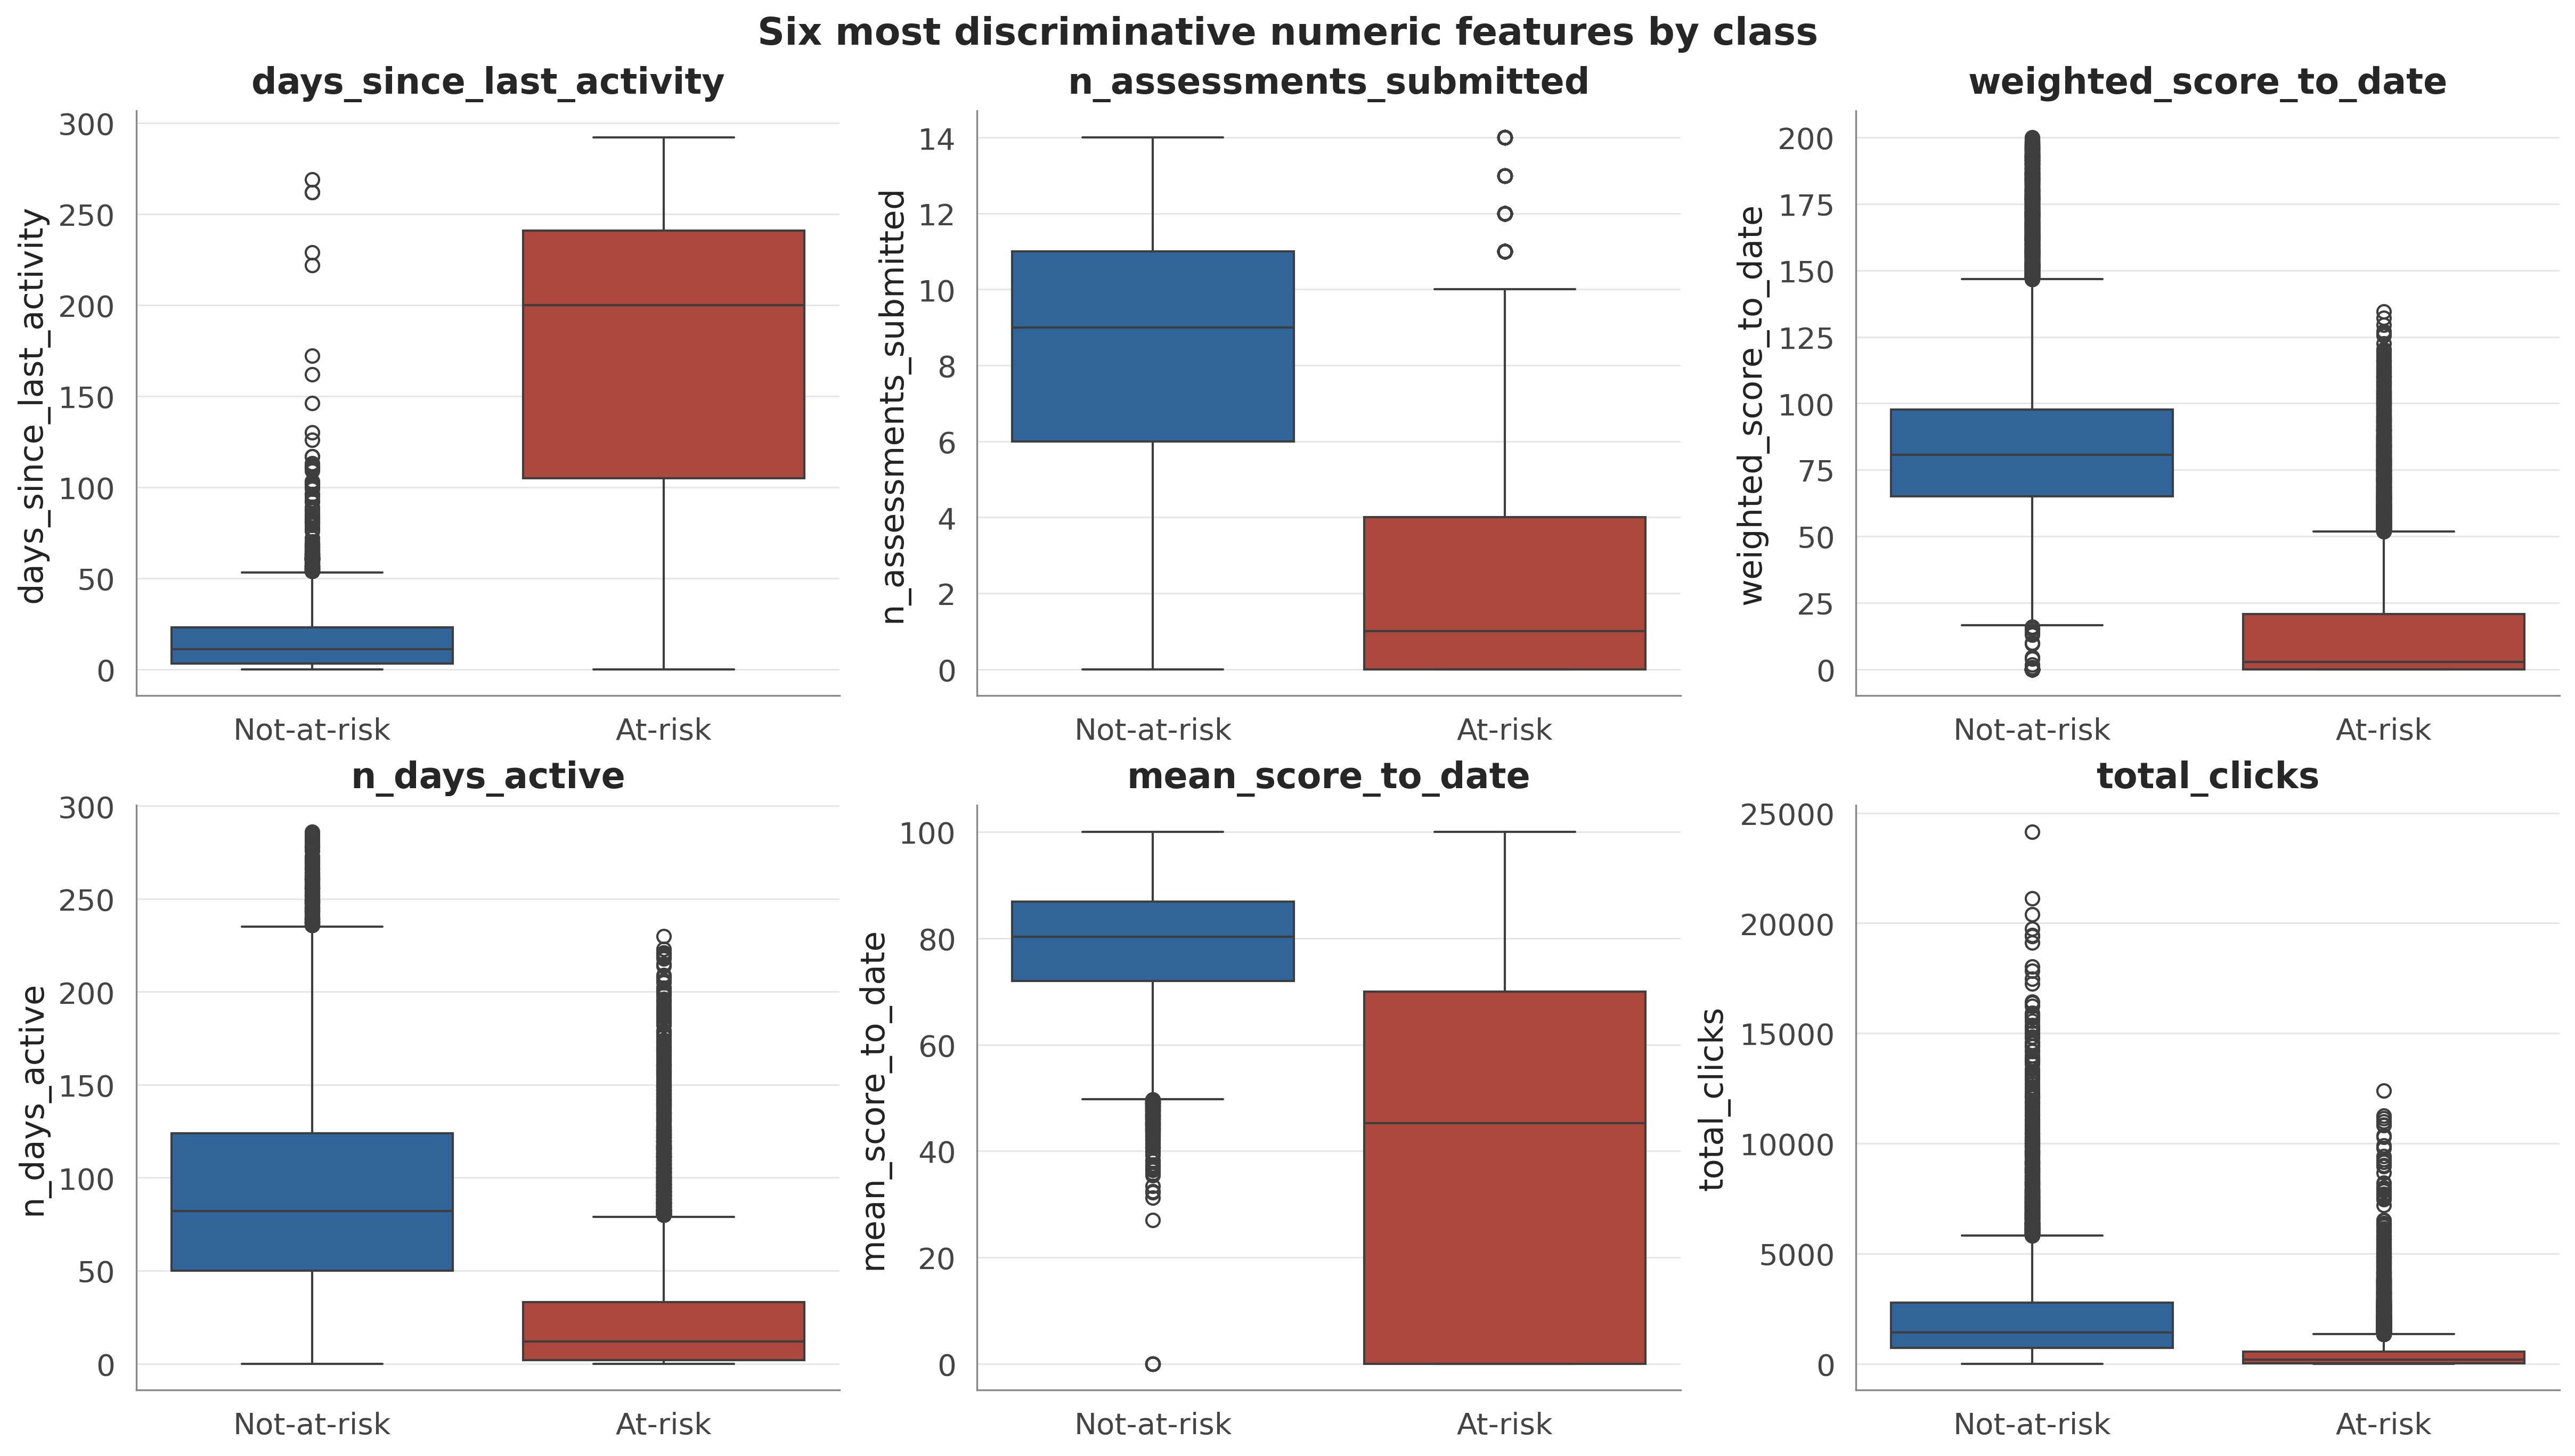
\includegraphics[width=\linewidth,height=0.80\textheight,keepaspectratio]{bivariate_top_boxplots.png}
\end{frame}

\begin{frame}{Categorical Features vs At-Risk (Cramér's $V$)}
  \begin{columns}[T]
    \begin{column}{0.6\textwidth}\centering
      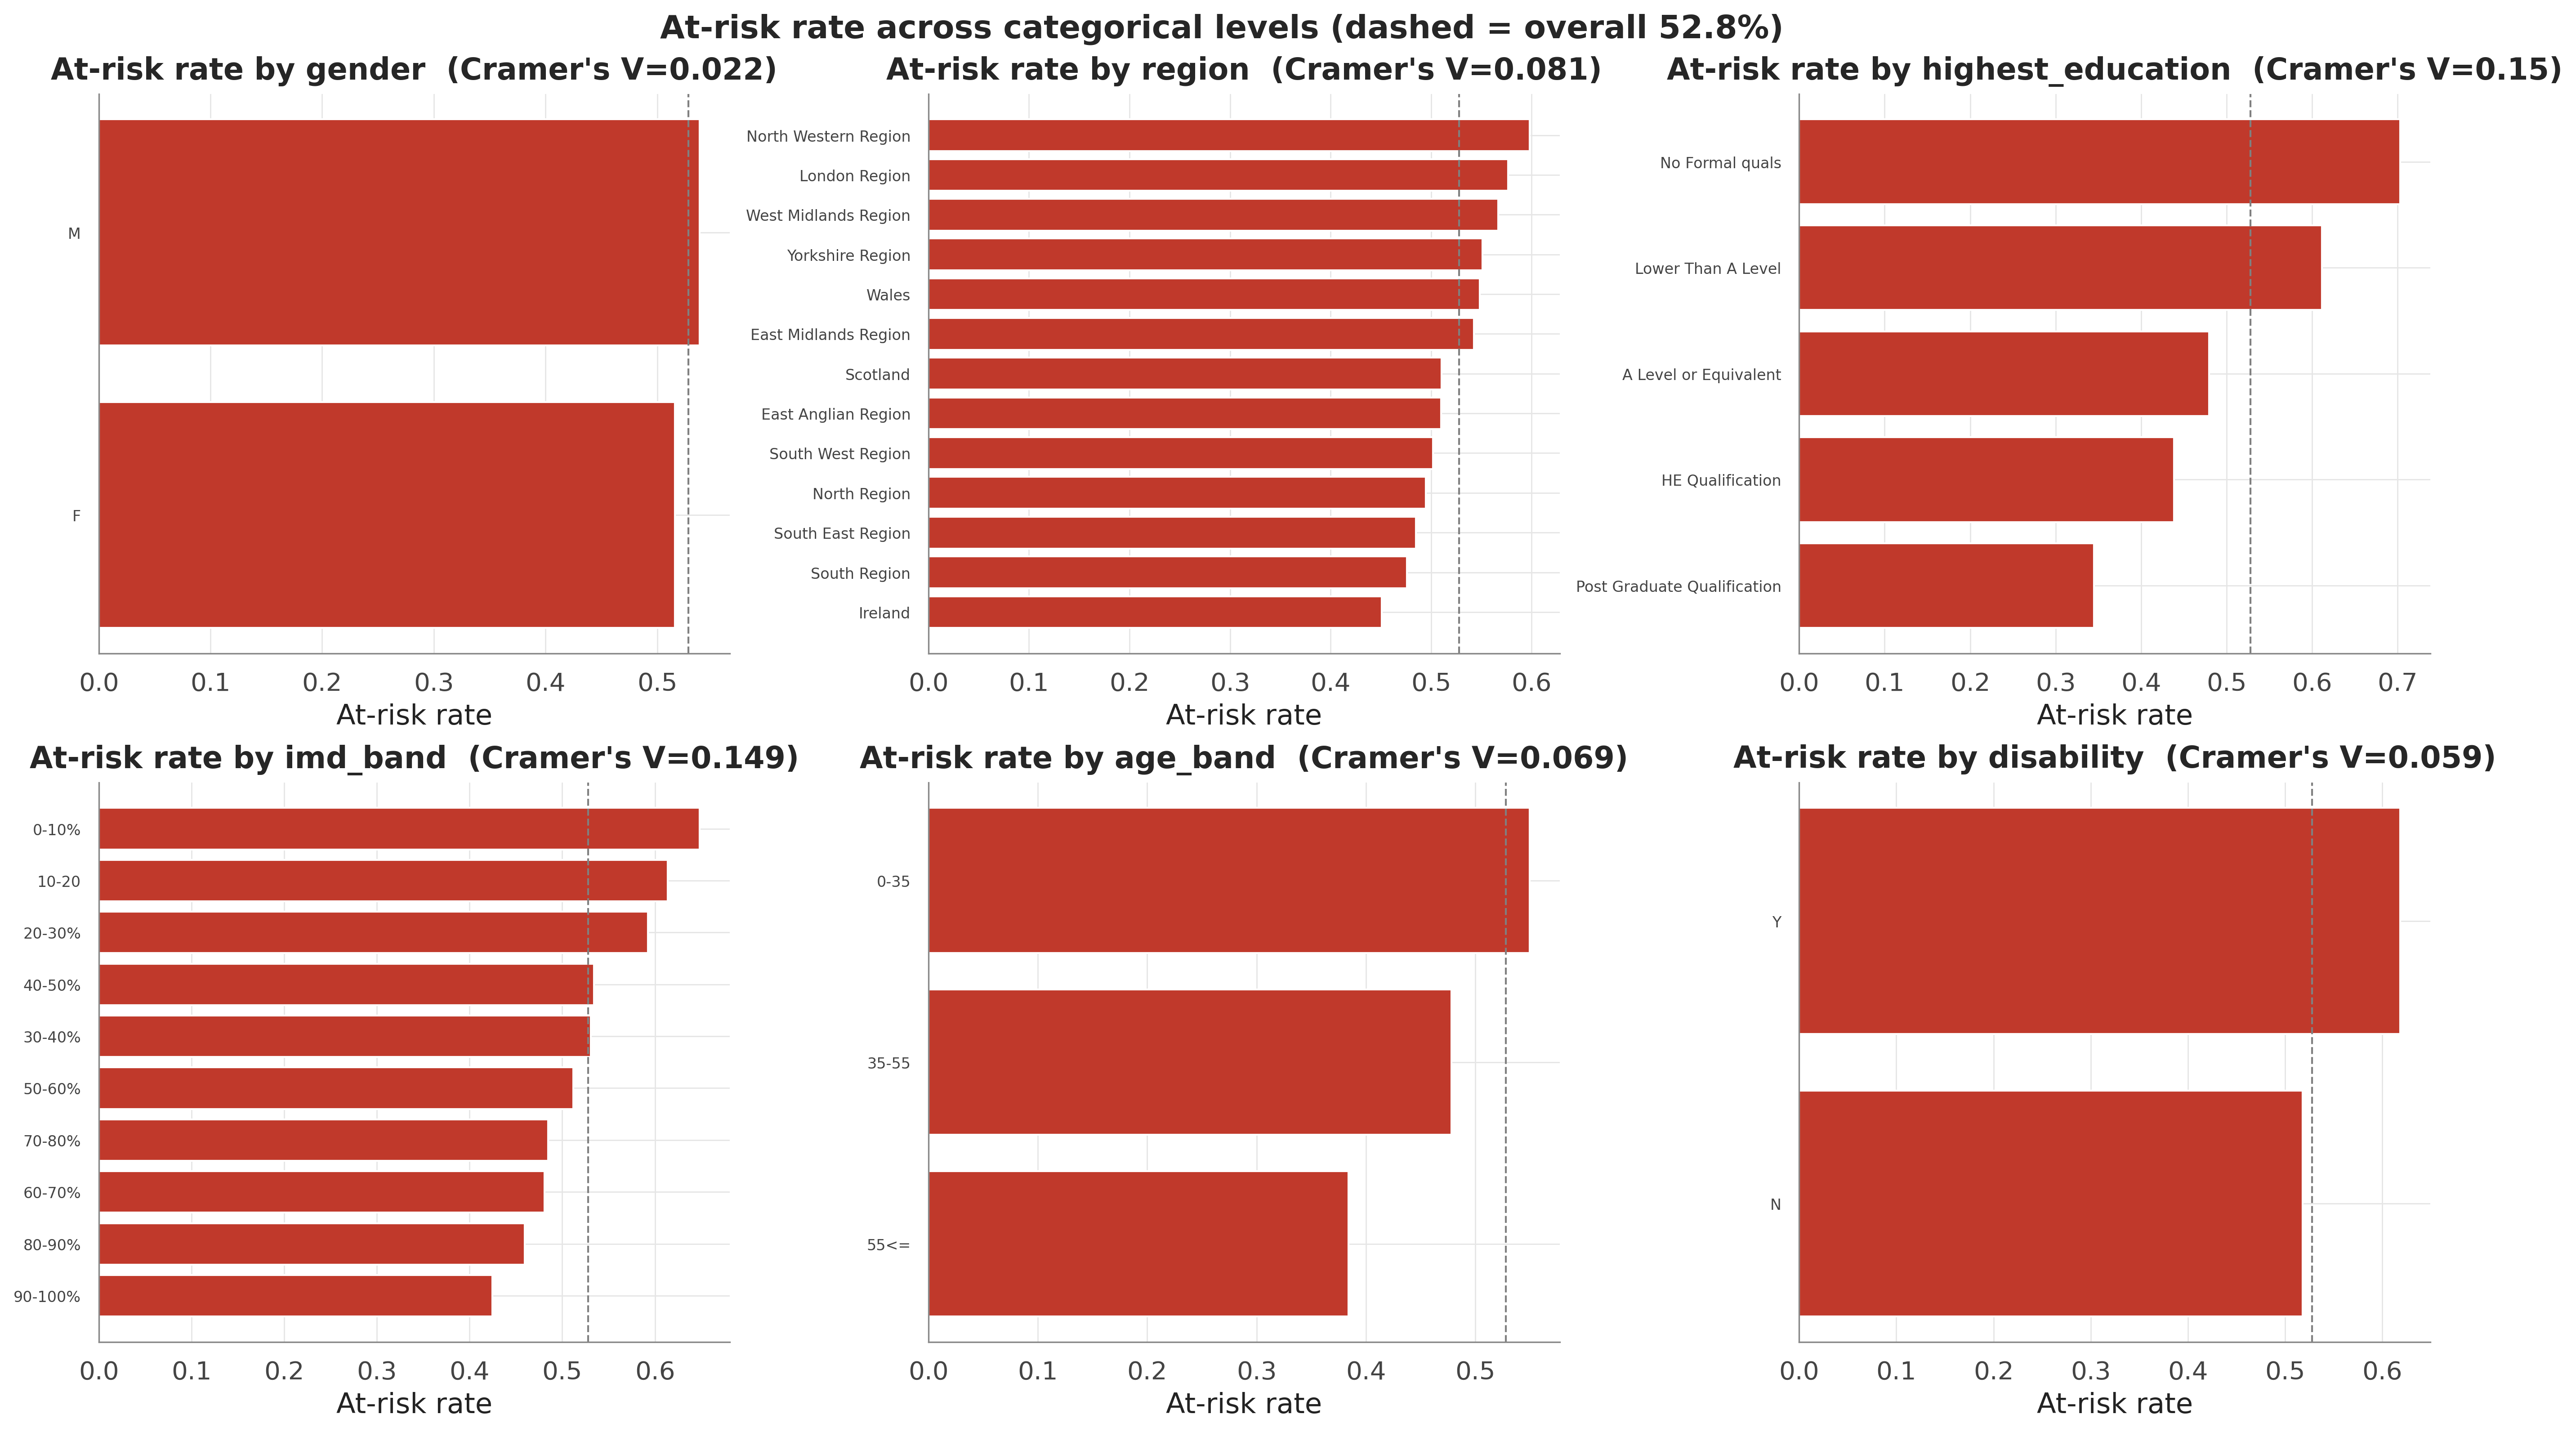
\includegraphics[width=\linewidth,height=0.78\textheight,keepaspectratio]{bivariate_categorical_rate.png}
    \end{column}
    \begin{column}{0.4\textwidth}\footnotesize
      \begin{itemize}\setlength\itemsep{0.3em}
        \item All significant, but associations are \textbf{weak}: $V\leq$ \textcolor{ccnured}{0.15}.
        \item Strongest: \tcode{highest\_education} \& \tcode{imd\_band} (0.15); \tcode{gender} negligible (0.02).
        \item Keep demographics for \textbf{fairness} analysis, not prediction.
      \end{itemize}
      \takeaway{Demographic effect ($V\leq0.15$) $\ll$ behavioural effect ($d$ up to 2.55).}
    \end{column}
  \end{columns}
\end{frame}

% =====================================================================
\section{Multivariate Analysis}
% =====================================================================
\begin{frame}{Correlation \& Multicollinearity}
  \begin{columns}[T]
    \begin{column}{0.58\textwidth}\centering
      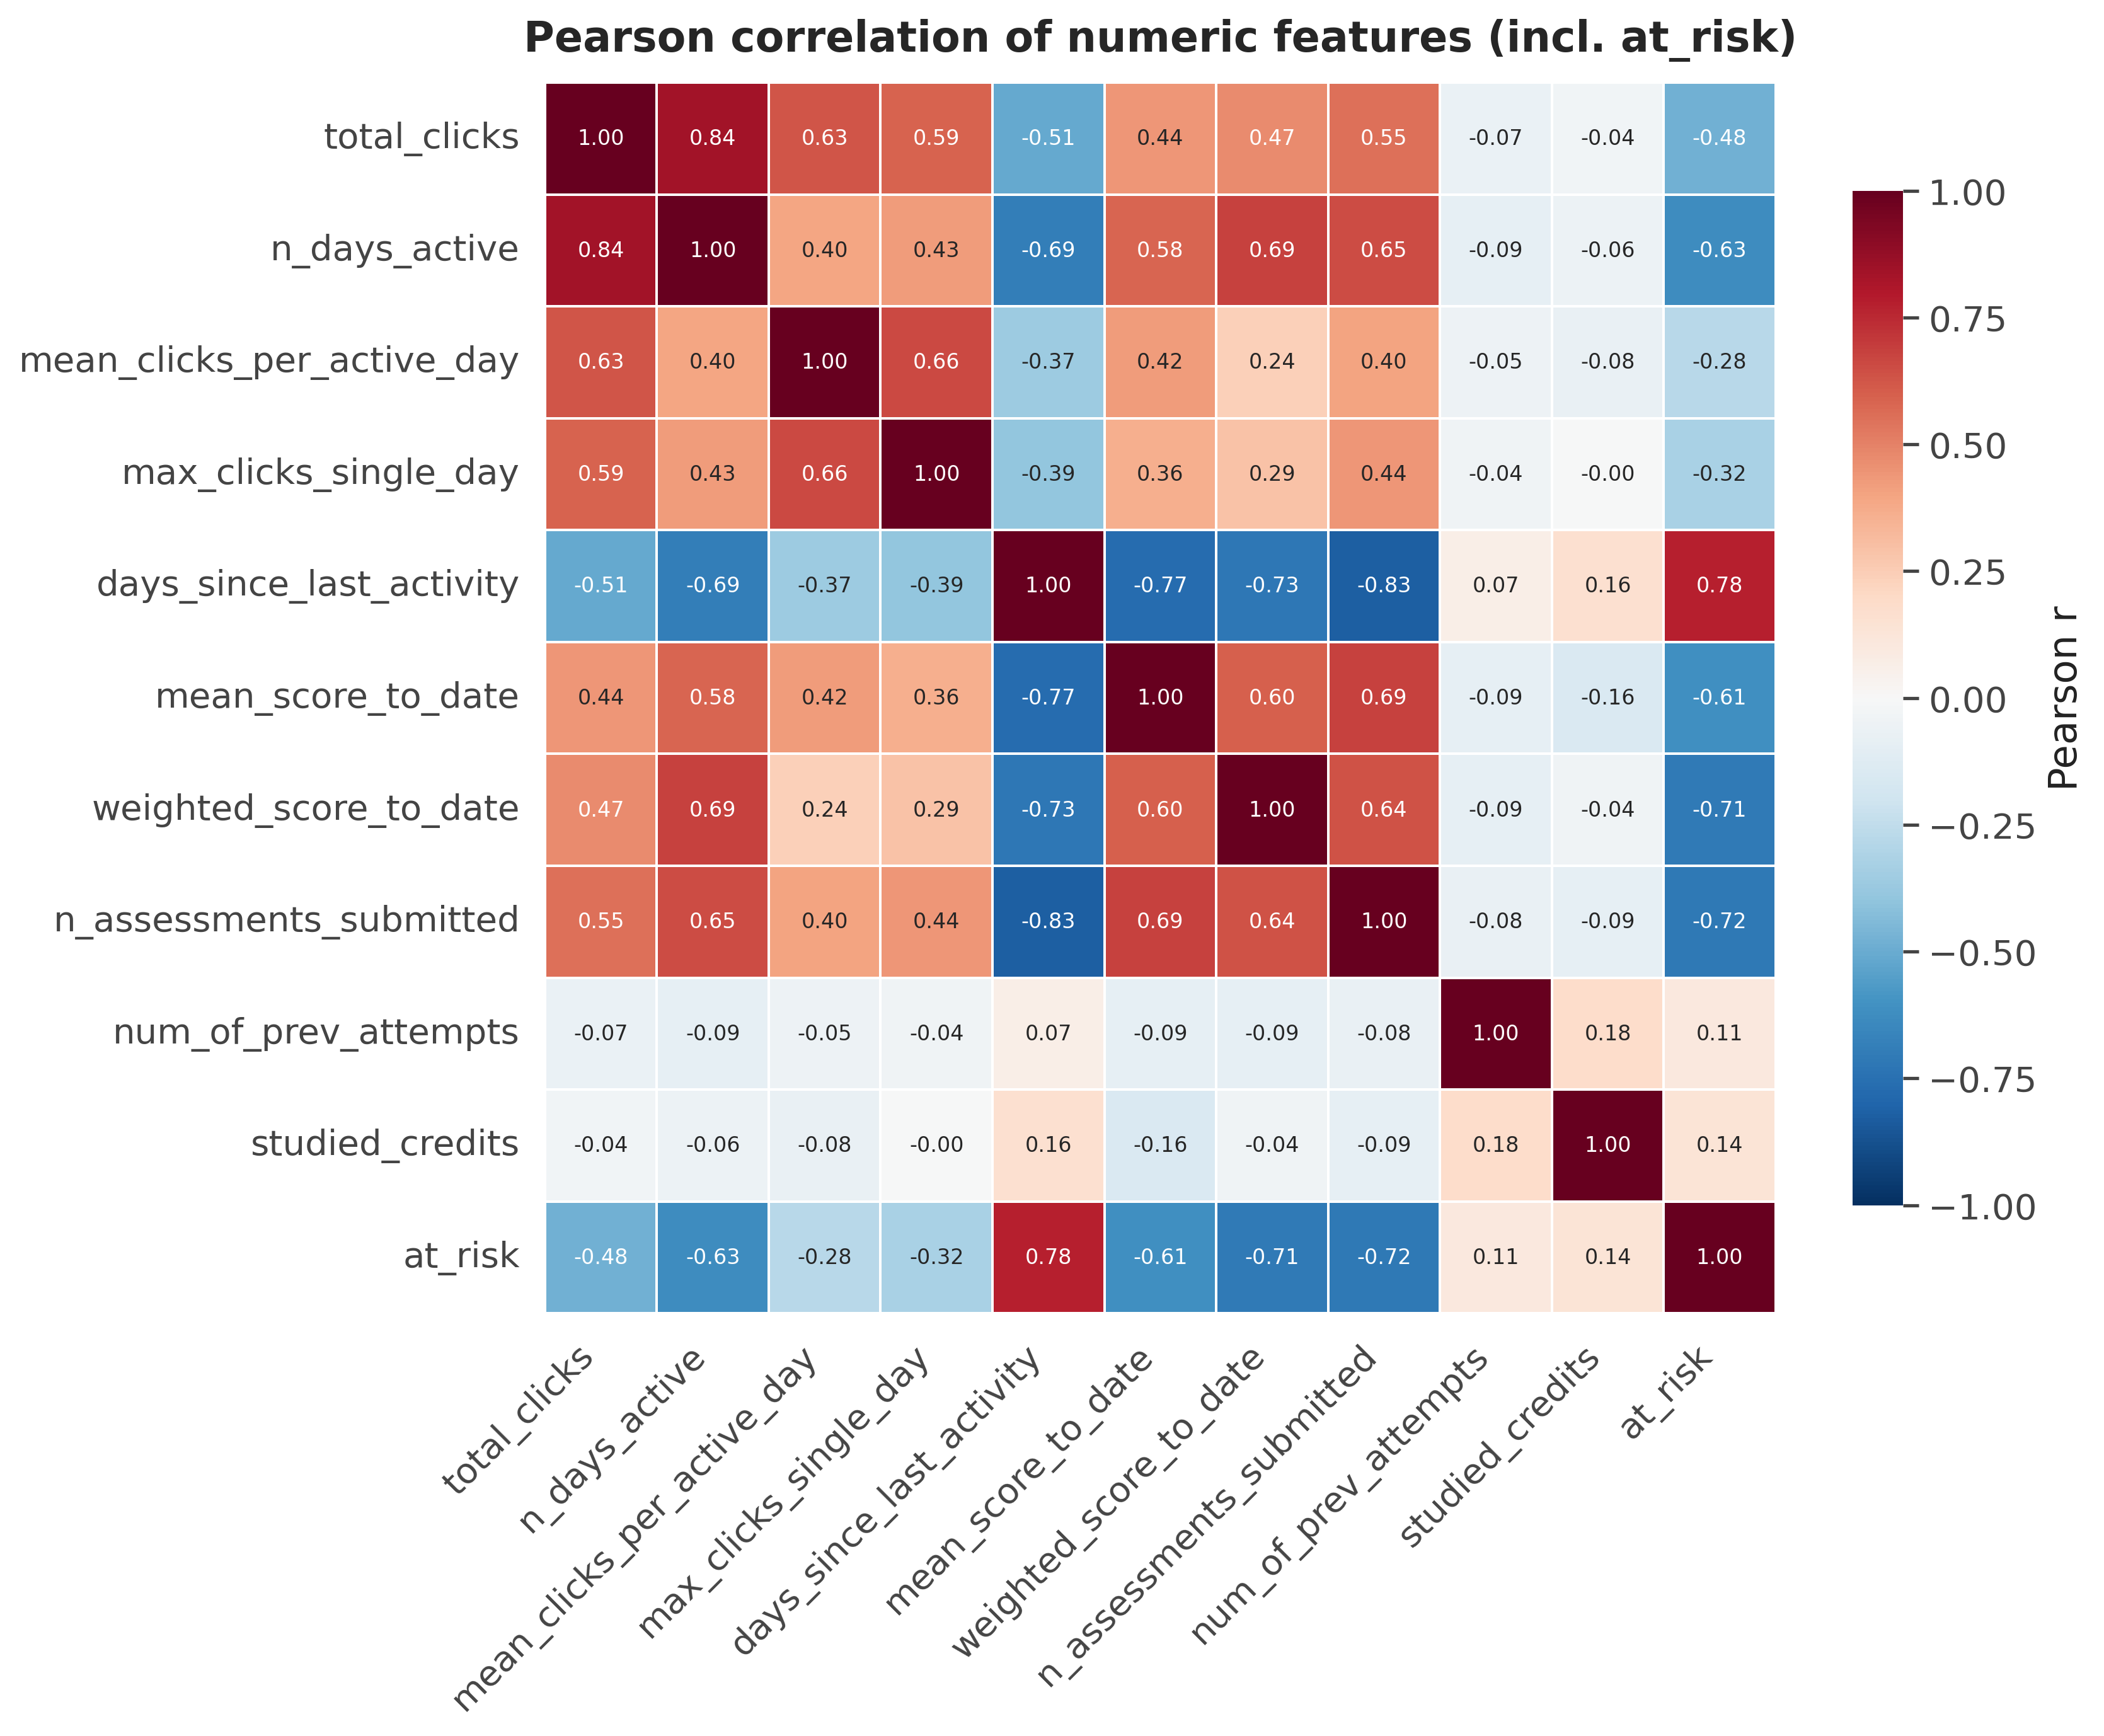
\includegraphics[width=\linewidth,height=0.78\textheight,keepaspectratio]{corr_pearson.png}
    \end{column}
    \begin{column}{0.42\textwidth}\footnotesize
      \begin{itemize}\setlength\itemsep{0.3em}
        \item Pearson (linear) + Spearman (monotonic) agree on the structure.
        \item Two multicollinear pairs $|r|\geq0.8$: \tcode{n\_days\_active}–\tcode{total\_clicks} (0.84), \tcode{days\_idle}–\tcode{n\_assessments} ($-$0.83).
        \item Flagged for \textbf{RQ2} — SHAP/LIME may split importance among correlated features.
      \end{itemize}
    \end{column}
  \end{columns}
\end{frame}

\begin{frame}{Correlation with the Target \& Leakage Check}
  \begin{columns}[T]
    \begin{column}{0.56\textwidth}\centering
      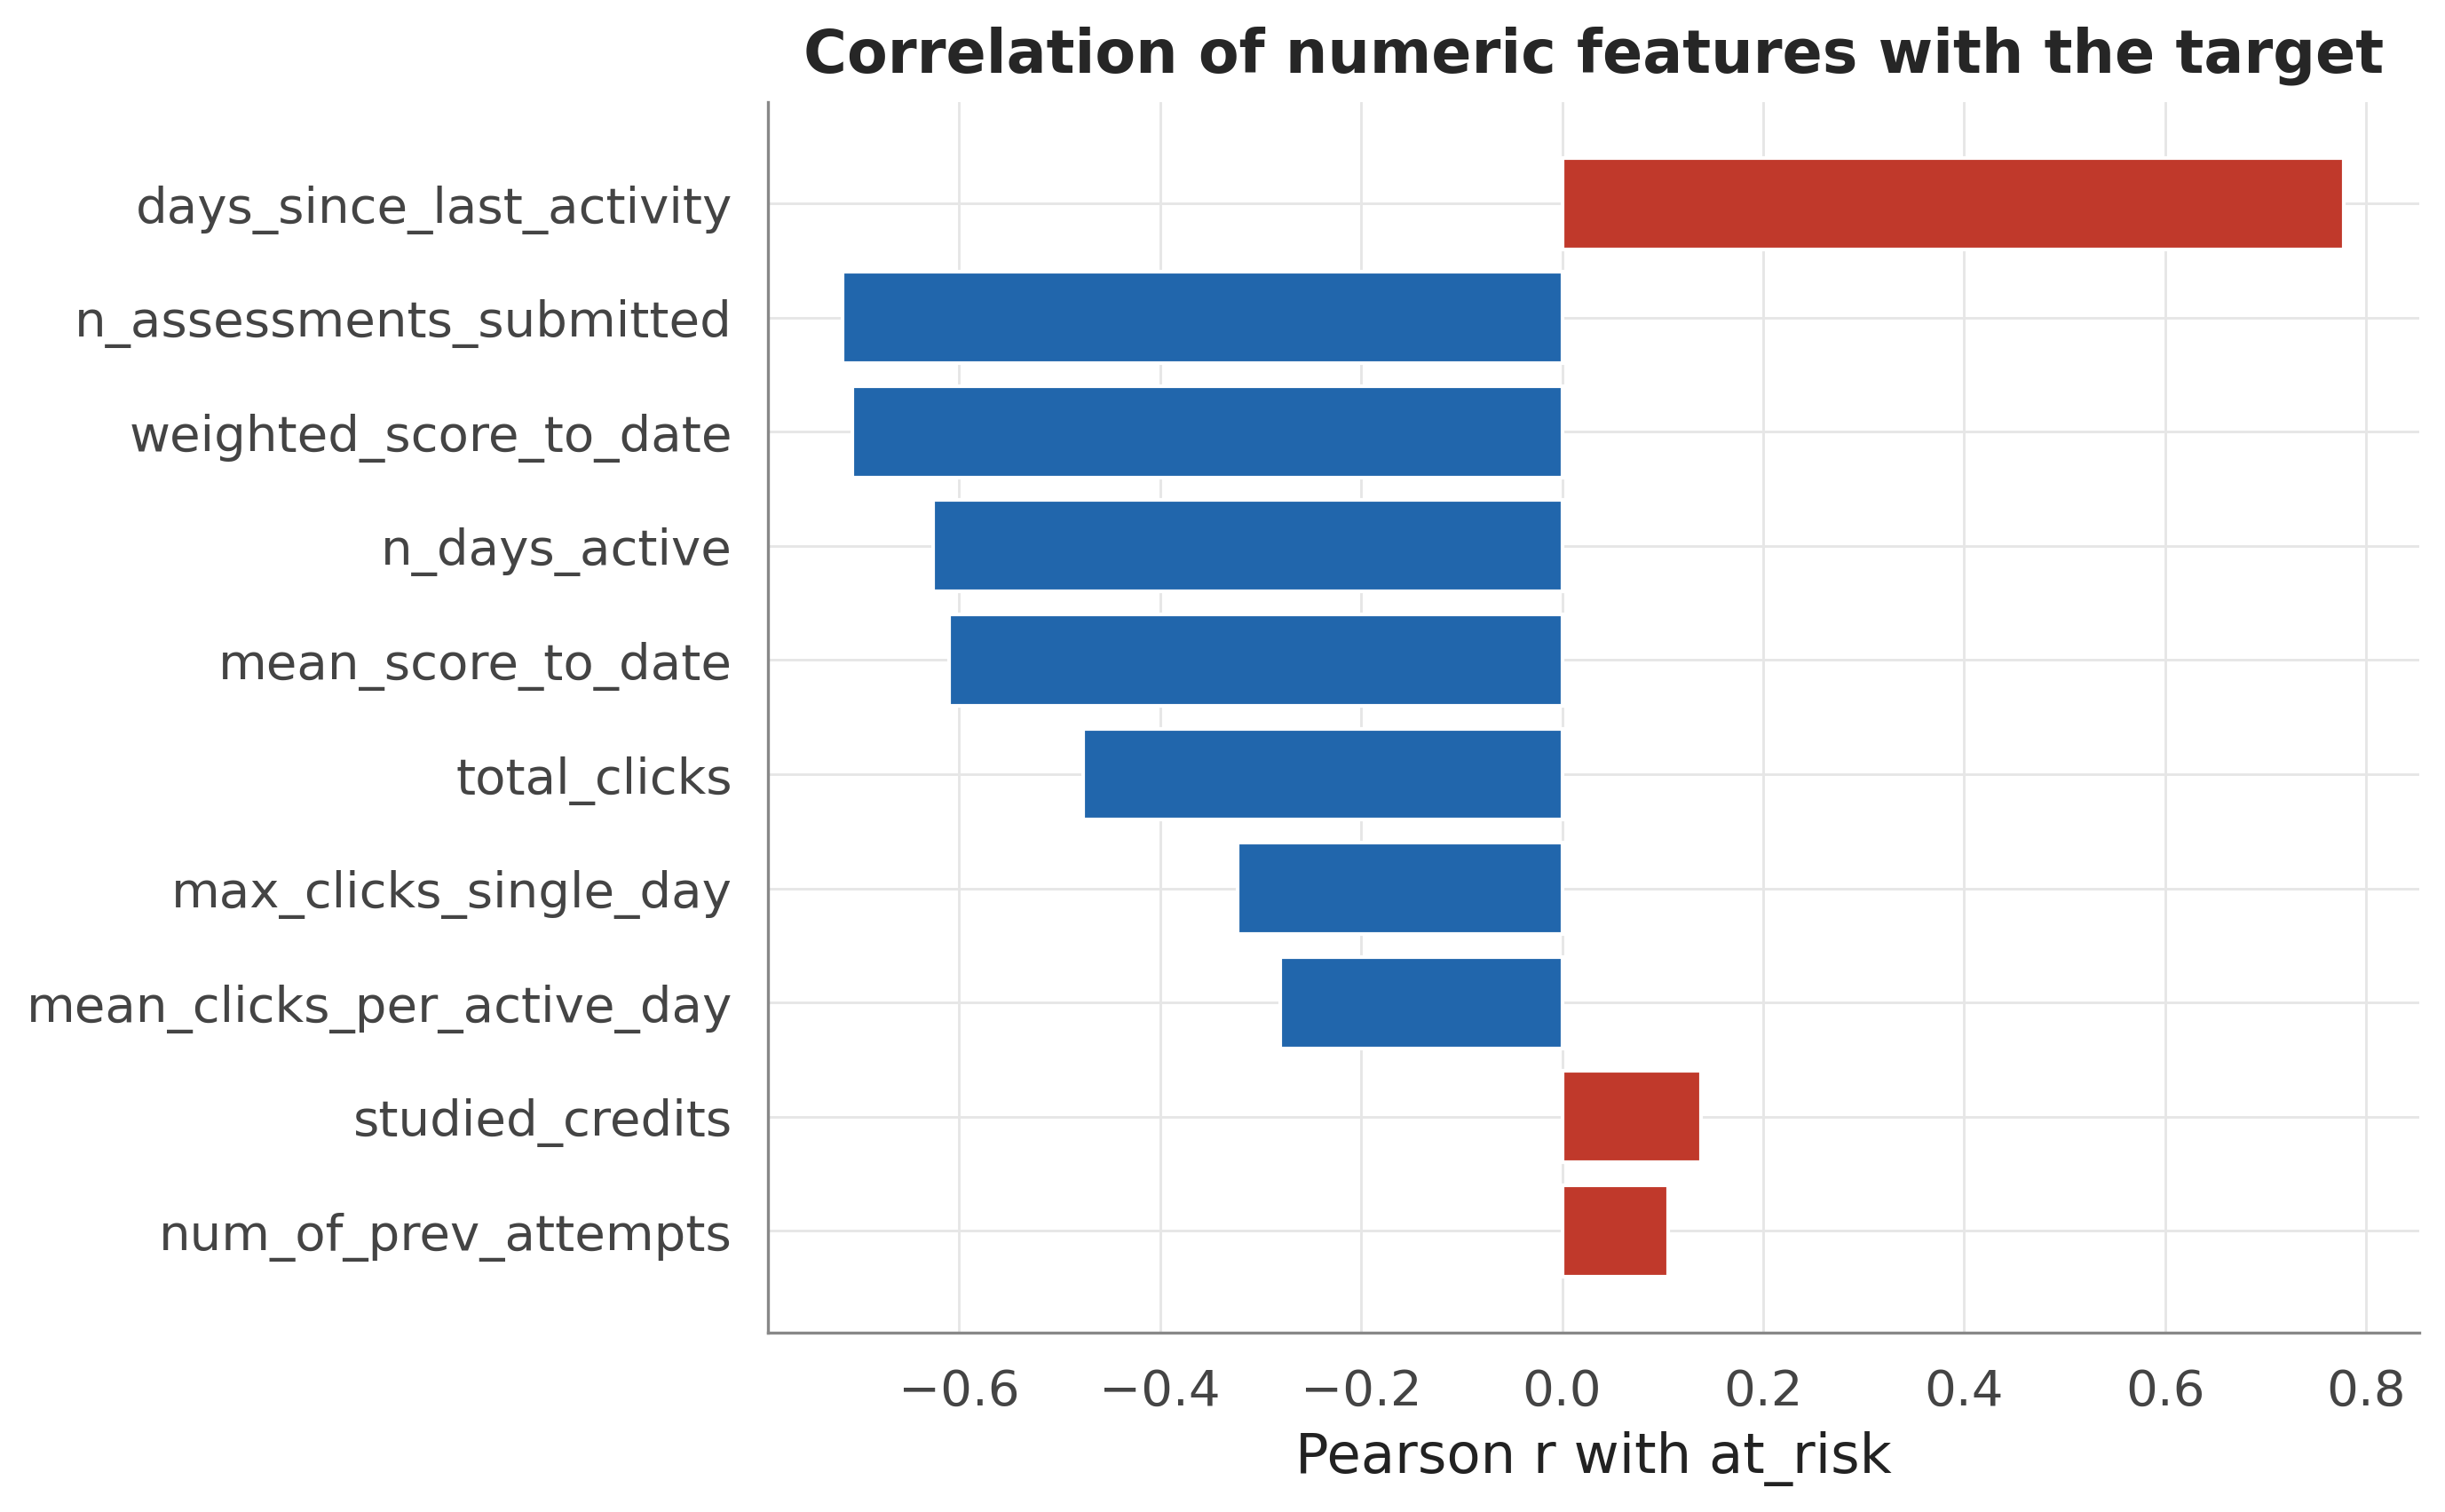
\includegraphics[width=\linewidth,height=0.78\textheight,keepaspectratio]{corr_with_target.png}
    \end{column}
    \begin{column}{0.44\textwidth}\footnotesize
      \begin{itemize}\setlength\itemsep{0.3em}
        \item Top $|r|$ with label: \tcode{days\_idle} \textcolor{ccnured}{+0.78}, \tcode{n\_assessments} $-$0.72, \tcode{weighted\_score} $-$0.71.
        \item Matches the Cohen's $d$ ranking — two independent methods, same conclusion.
        \item \textbf{No feature $|r|\geq0.95$} $\Rightarrow$ no leakage suspect.
      \end{itemize}
      \takeaway{The leakage check here is the EDA half of the anti-leakage guarantee tested in the split stage.}
    \end{column}
  \end{columns}
\end{frame}

% =====================================================================
\section{Time-Aware Analysis (RQ1)}
% =====================================================================
\begin{frame}{When Does the Signal Emerge?}
  \begin{columns}[T]
    \begin{column}{0.56\textwidth}\centering
      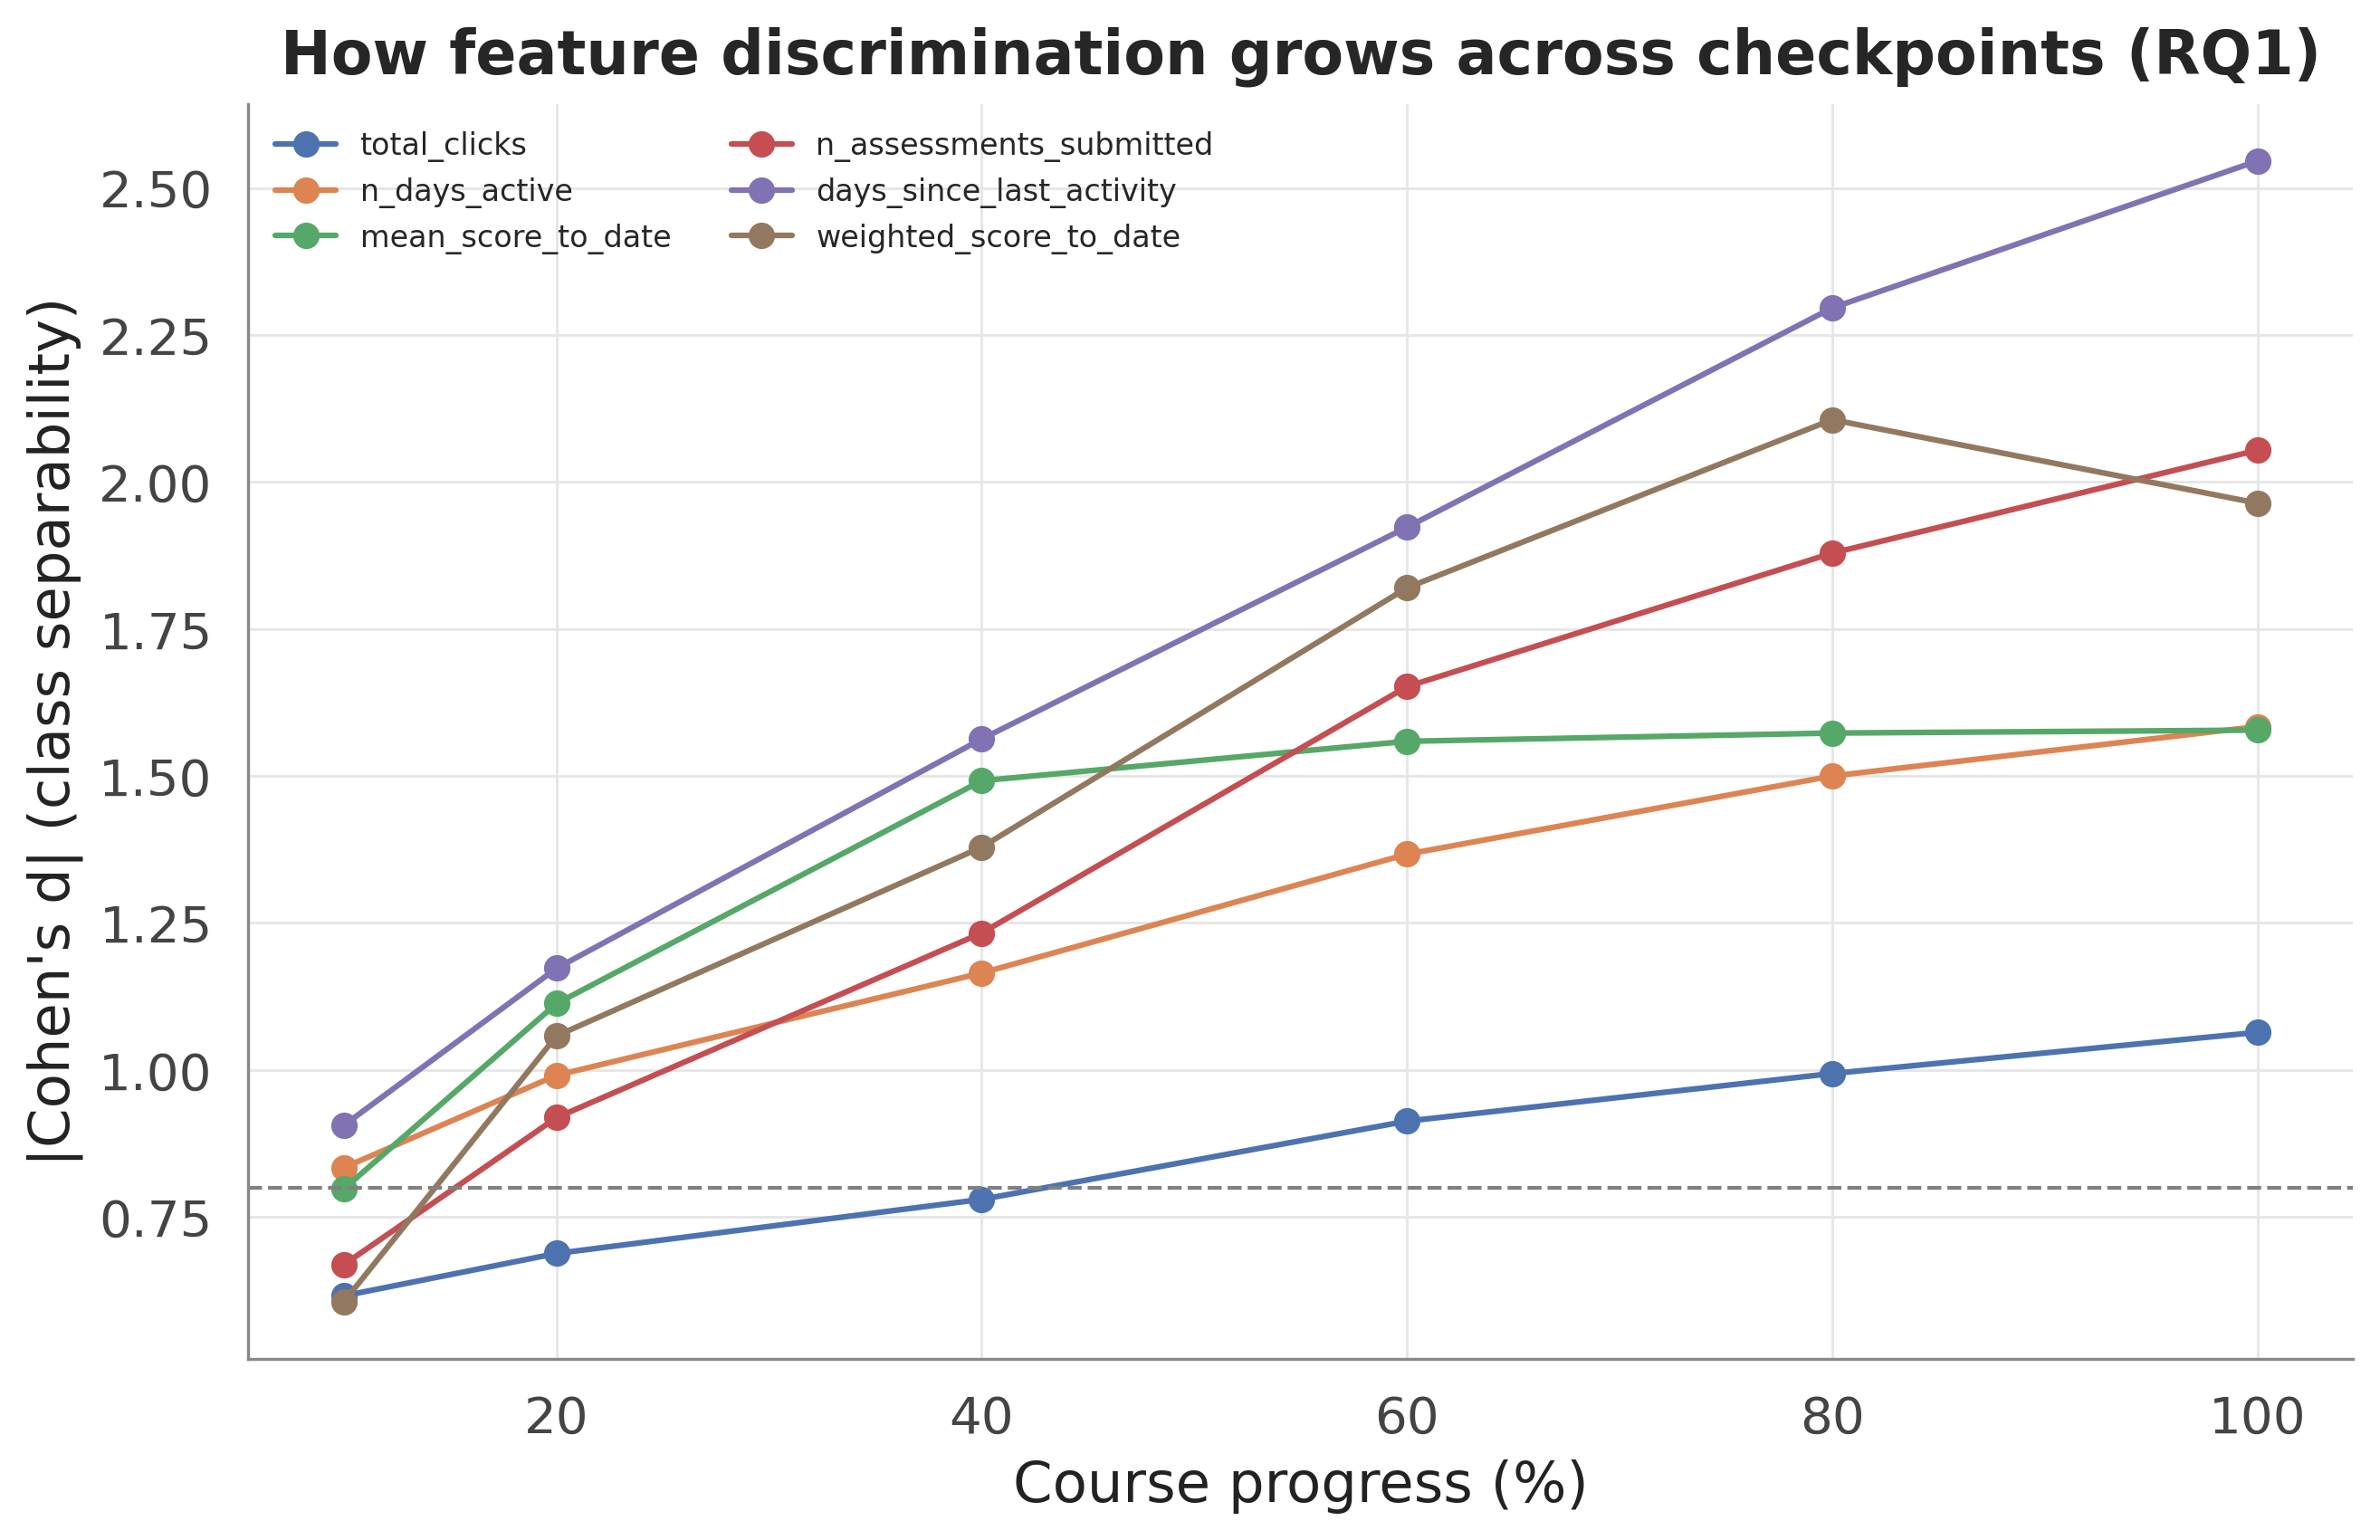
\includegraphics[width=\linewidth,height=0.78\textheight,keepaspectratio]{time_discrimination_curve.png}
    \end{column}
    \begin{column}{0.44\textwidth}\footnotesize
      \begin{itemize}\setlength\itemsep{0.3em}
        \item |Cohen's $d$| per feature across the \textbf{6 checkpoints} (10\%$\to$100\%); discrimination \textbf{grows steadily}.
        \item First to reach $d\geq0.8$: \tcode{n\_days\_active} \textbf{and} \tcode{days\_since\_last\_activity} from \textbf{10\%}; scores/submissions from \textbf{20\%}.
      \end{itemize}
      \keynum{early prediction feasible from \textbf{$\sim$10–20\%} — this sets the RQ1 checkpoint schedule.}
    \end{column}
  \end{columns}
\end{frame}

\begin{frame}{Mean Trajectory by Class}
  \centering
  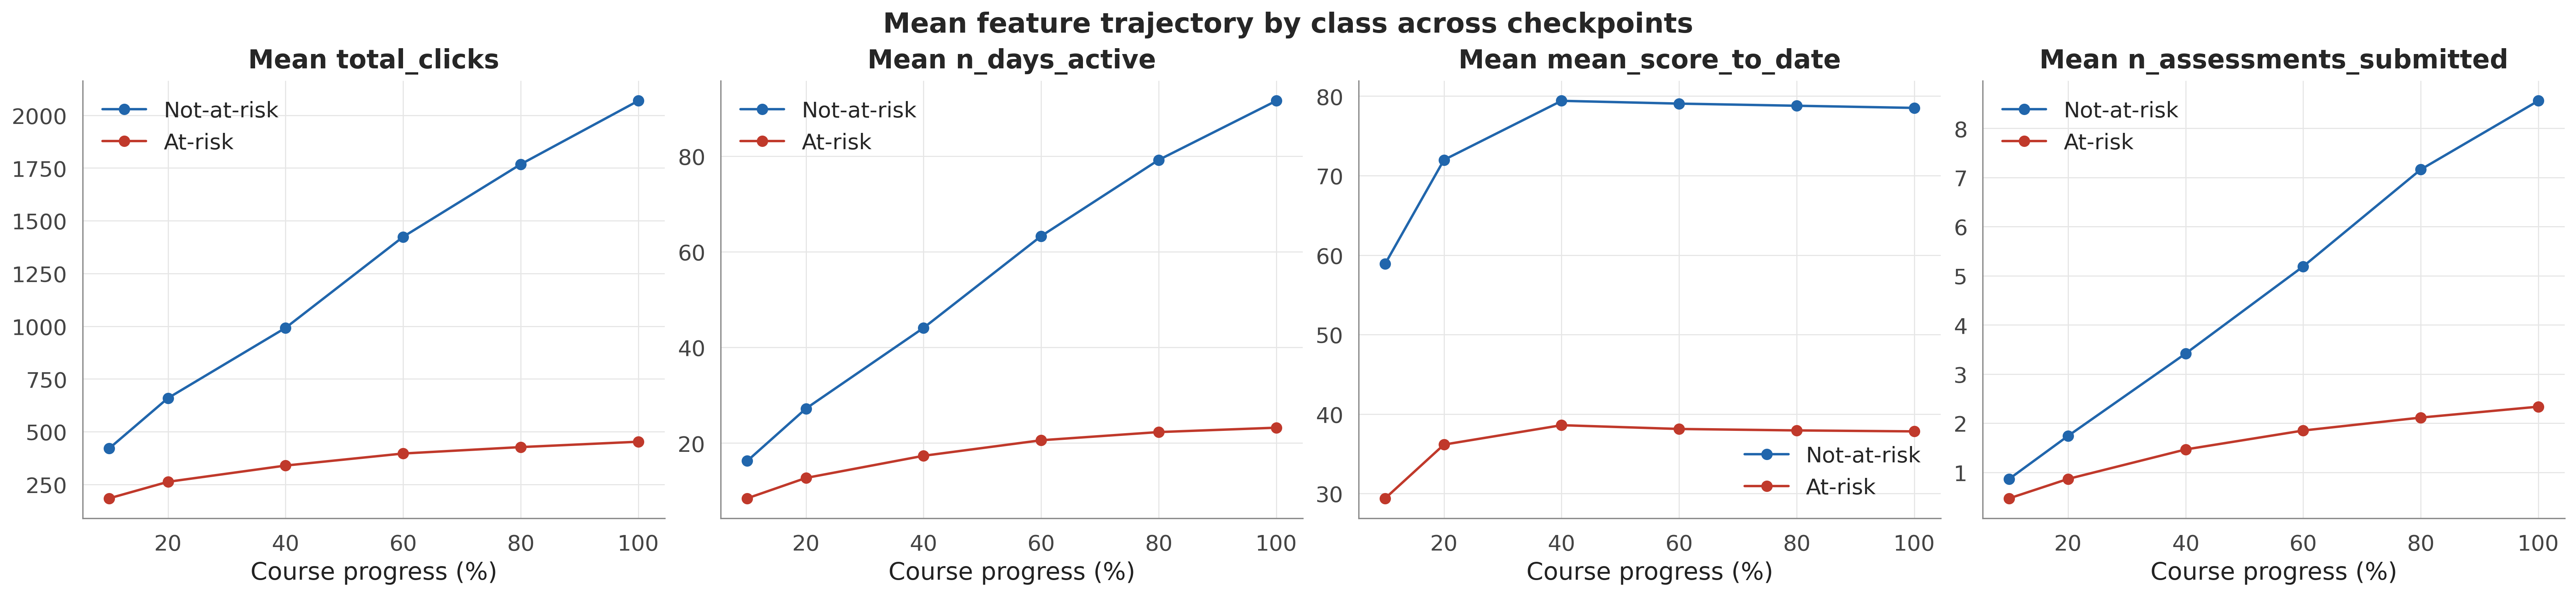
\includegraphics[width=\linewidth,height=0.80\textheight,keepaspectratio]{time_mean_trajectory.png}
\end{frame}

\begin{frame}{The Withdrawn Early-Warning Signal}
  \begin{columns}[T]
    \begin{column}{0.56\textwidth}\centering
      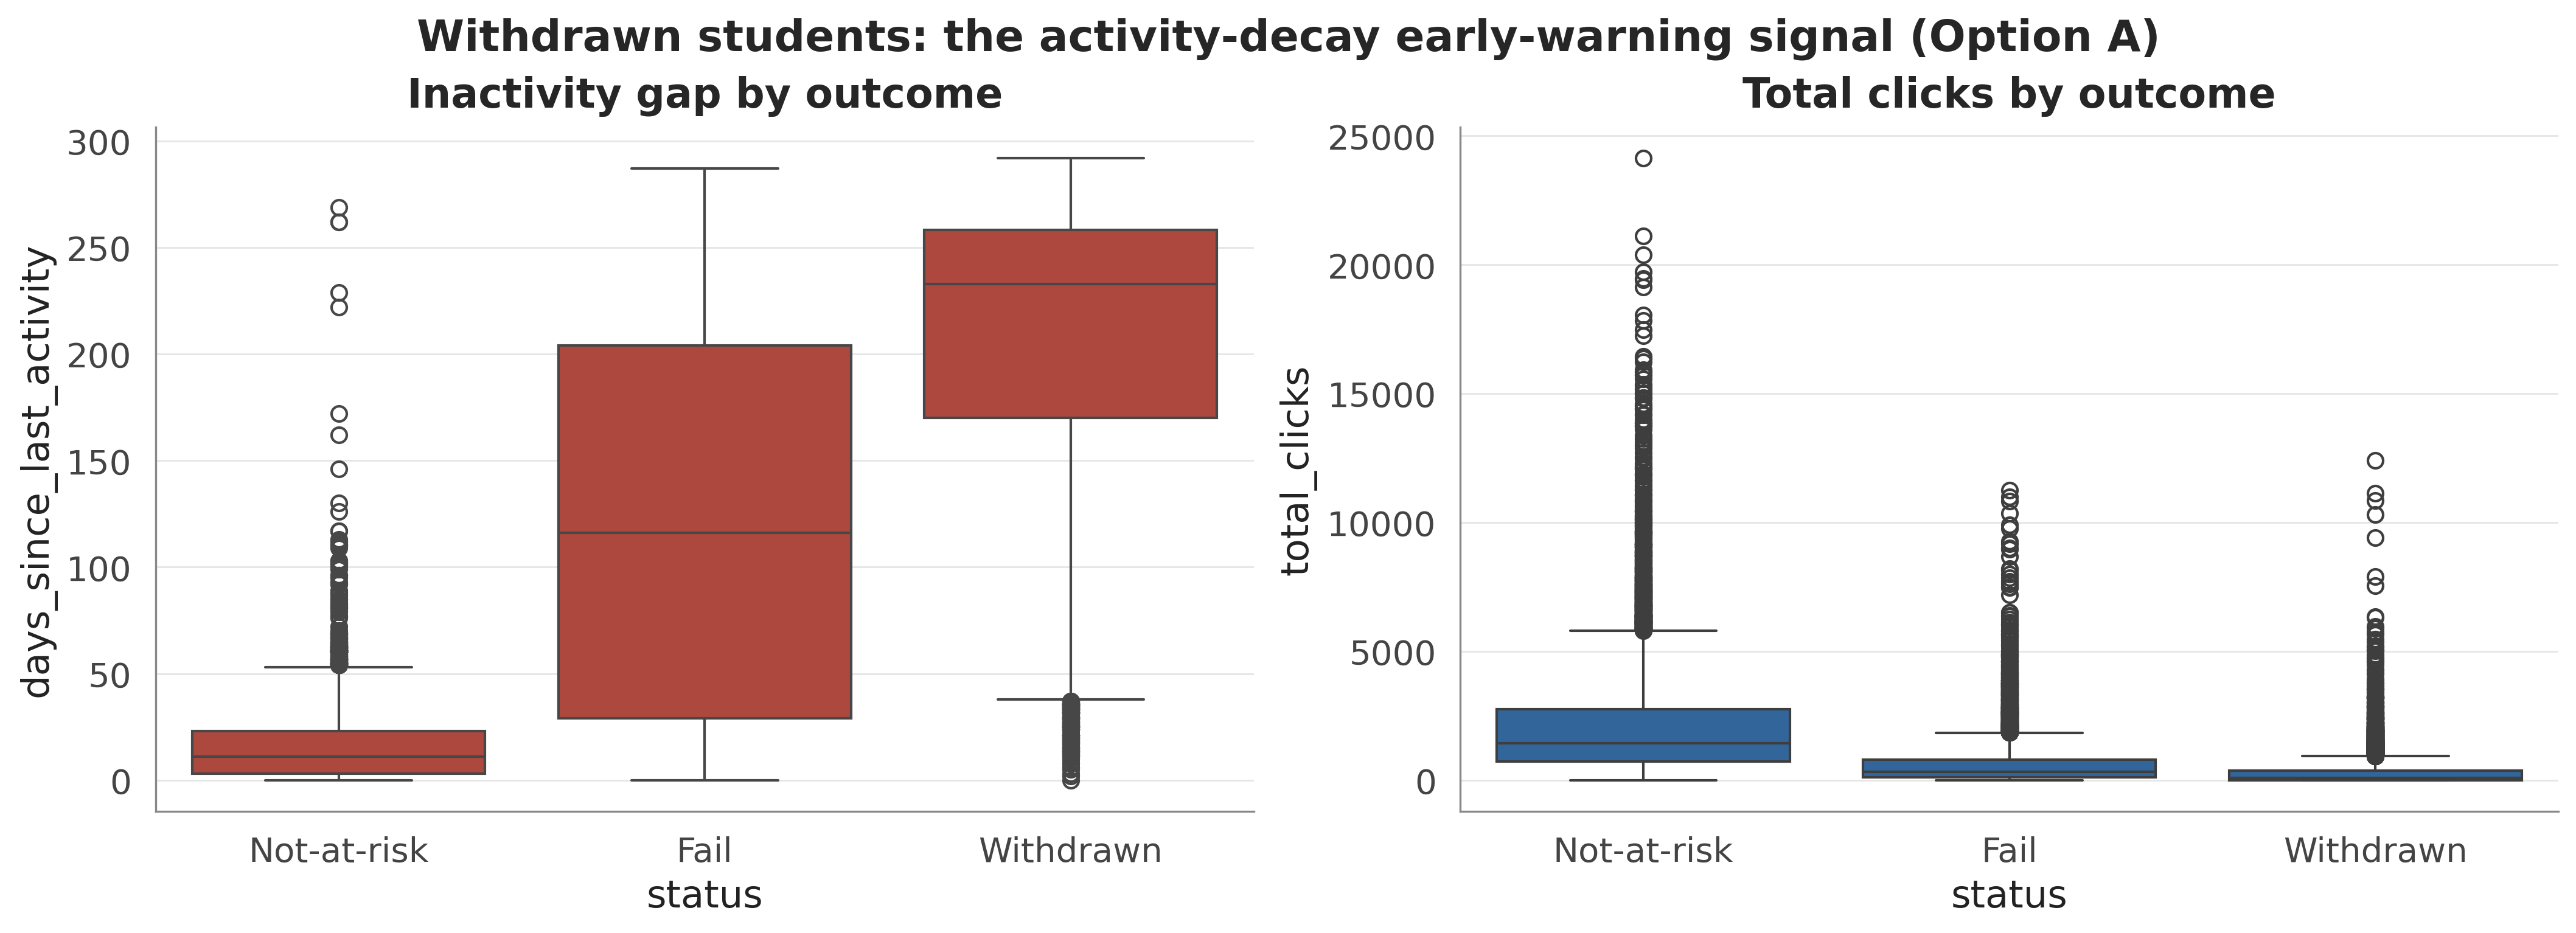
\includegraphics[width=\linewidth,height=0.74\textheight,keepaspectratio]{withdrawn_activity_decay.png}
    \end{column}
    \begin{column}{0.44\textwidth}\footnotesize
      \begin{itemize}\setlength\itemsep{0.3em}
        \item Median days idle: \textbf{11} (not-at-risk) $\to$ 116 (Fail) $\to$ \textbf{233} (Withdrawn); median clicks $\sim$1,425 $\to$ 89.
        \item A genuine signal — the activity collapse is what makes early detection feasible.
      \end{itemize}
      \takeaway{\textbf{Caveat:} withdrawn students are trivially separable \emph{late} $\Rightarrow$ the honest test is the \emph{early} checkpoints.}
    \end{column}
  \end{columns}
\end{frame}

% =====================================================================
\section*{Conclusion}
% =====================================================================
\begin{frame}{EDA — Findings \& Implications}
  \footnotesize
  \begin{itemize}\setlength\itemsep{0.45em}
    \item \textbf{Distributions:} clickstream strongly right-skewed (up to 34.7) $\Rightarrow$ \tcode{log1p}; \tcode{days\_idle} bimodal.
    \item \textbf{Behaviour $\gg$ demographics (RQ1/RQ2):} Cohen's $d$ up to \textbf{2.55}; all 19 numeric significant; Cramér's $V\leq0.15$.
    \item \textbf{No leakage:} no $|r|\geq0.95$; 2 multicollinear pairs flagged for SHAP stability.
    \item \textbf{Early signal (RQ1):} usable from \textbf{$\sim$10–20\%} of course length; 40–60\% is a robust window.
    \item \textbf{Mild imbalance (RQ3):} 52.8\% at-risk $\Rightarrow$ PR-AUC/recall; resampling on train only.
  \end{itemize}
  \takeaway{EDA hands the rest of the pipeline: what to transform, which features carry signal, that there is no leakage, and when to predict.}
\end{frame}

\begin{frame}[plain]{Thank you}
  \vfill\centering
  {\Huge\textcolor{ccnured}{Thank you}}\\[1.0em]
  {\footnotesize\textbf{Key references}}\\[0.3em]
  {\scriptsize
   Kuzilek, Hlosta, Zdrahal (2017), \emph{OULAD}, Scientific Data 4:170171.\quad
   Adnan et al.\ (2021), \emph{IEEE Access} 9.\quad Tomasevic et al.\ (2020), \emph{Computers \& Education} 143.}
  \vfill
\end{frame}

\end{document}
